%% Before beginning to type your dissertation, read the formatting guide, 
%% which can be found at http://grad.msu.edu/etd/docs/formattingguide.pdf
%% Also get the latest version of  msuphddissertation.cls and the template file
%% at http://www.math.msu.edu/~weil/MSU_Ph.D._Dissertation.zip
%% Send questions to weil@math.msu.edu
\documentclass{msuphddissertation}
\usepackage{amssymb, amsmath}
\usepackage{natbib}
%\usepackage{subcaption}
\usepackage{graphicx}
\usepackage{url}
%% Insert packages you wish to use except setspace and subfig. 
%% Those packages are loaded automatically.
%% IMPORTANT: Load only those packages you know you will use.
%% Some packages can cause conflicts resulting in improper formatting.
\author{Elijah K. Lowe} %% Put your name in full as it is officially recognized by Michigan State University here.
\title{The wood chipper problem: } %% Put the title of your dissertation here.
\unit{Computer Science \& Engineering} %% Put the name of your degree granting unit here. The complete
%% list of these degree granting units can be found at
%% http://grad.msu.edu/etd/docs/DegreeGrantingUnits.pdf

%% Put additional preamble items here.

%%%%%% LANDSCAPE PAGES  %%%%%%
%% The environment, landscapenum, produces a page in 
%% landscape mode and then rotates the page by 90 degrees 
%% making is readable on a computer screen, and places the page number
%% along the 11 inch side, which is the bottom of the rotated page. 

%%%%%%%%%%%%%%%%%%%%%%%%%%%%
%%%%%%%%  NOTE   %%%%%%%%%%%%%%
%% PREPARING A DISSERTATION WITH THIS CLASS FILE DOES NOT %%%
%% GUARANTEE THAT THE GRADUATE SCHOOL WILL APPROVE IT %%%
%%%%%%%%%%%%%%%%%%%%%%%%%%%%%%%

%%%%%%%%%%%%%%%%%%%%%%%%%%%%%%%%%%
%%%%%%%%%%%% WARNING %%%%%%%%%%%%%%%
%% The Graduate School requires that all text, except superscripts %%
%% and subscripts, but including text in imported %%
%% graphics files be in 12 point. For that reason it's recommended %%
%% that no text be part of any imported files. %%

%% Once your document has been filed with the Graduate School,
%% if you wish to produce a version of it whose subscripts and superscripts
%% are in traditional smaller proportion, remove the "%" sign 
%% in front of following command. 
%\DeclareMathSizes{12}{12}{10}{8}
%% If your document has footnotes, remove the "%" sign 
%% in front of following command. 
%\renewcommand{\footnotesize}{\small}
%% To single space your document, remove the 
%% two commands \begin{doublespace}
%% and \end{doublespace} below.

\begin{document}

\maketitlepage %%This command will produce the title page of your thesis.
\begin{abstract}
Abstract goes here
\end{abstract}

%% If you wish to have a copyright page, remove the "%" in front of  \begin{copyrt}
%% and remove the "%" in front of \end{copyrt}.
%% The mandatory form of the Copyright will be generated automatically. 
%% A copyright statement is optional.

%\begin{copyrt}
%\end{copyrt}
%% If you wish to have a dedication, remove the "%" in front of
%% \begin{dedication}
%% \end{dedication}
%% A dedication must be single-spaced and 
%% centered on the page.  Both will be done automatically. 

\begin{dedication}
\begin{center} 

\end{center}
\end{dedication}

%% If you wish to have an acknowledgment, remove the "%" in front of  \begin{acknowledgment}
%% and remove the "%" in front of  \end{acknowledgment}  
\begin{acknowledgment}
Where do I begin? I am a summation of all the people that I have come in contact throughout my life. So, I would like to dedicate this text to some of the most influential people. 

I start with my mother Patricia Lowe who always encouraged me to pursue my wildest dreams. My father William Robertson, who thought me to question the world and to always pay attention to the small things. My brother Fard Lowe, who consistently served as an inspiration to me and someone I could count on. To my high school consoler, Kathy Giles-Harris and high school math teacher, Christopher Reese who both saw something special in me, and pushed me to pursue it. 

My brothers from Morehouse\textemdash Terron Ferguson, Ryan Shepard, John-Marcus Philips, Sean Brazier and Kelechi Kalu\textemdash who keep the laughs and good times rolling along my journey. You guys always made me feel cool, even though I'm a science nerd and that was your intent.
  
My MSU family, who are too many to name, but I'll name a few\textemdash my brother and sister, Cameron Khalfani Herman and Neem Serra, my best bud Ruby Carrillo, Dr. Barbara Thelamour, my mentor Judi Brown-Clark, my problem solvers Connie James and Darcie Zubek, Carmel Martin-Fairey, Daniel Couvrtier, Luis Zaman, Chad Byers, Temple Smith, James Kremer, okay I said a few, so I'll stop there. I needed you all along the way, through late nights of studying, endless laughs, awesome food, much needed pep talks and just being there to help me survive Michigan.

Collaborators and friends, Billie Swalla, her lab, Lionel Christiaen, his lab, Alberto Stolfi and the wonderful Princess Claudia Racioppi, who all helped me to develop as biologist, experimentally and thinking wise, and has adviser me along the way. I look forward to working with you all for years to come. 

My adviser, Titus Brown. I cannot thank you enough for guiding me along the way. I truly lucked up when I landed in your lab. You are a great scientist, adviser, mentor, and person, and this is the only time you'll hear (or more like read) me say this.

My awesome committee who were always been tough, but fair.
And to those who pursue knowledge not for the sake of notability but just make the world a better place.
\end{acknowledgment}

%% If you wish to have a preface, remove the "%" in front of  \begin{preface}
%% and remove the "%" in front of  \end{preface}  
%\begin{preface}
%% Type your acknowledgment here. An acknowledgment is optional.
%\end{preface}

\TOC

%% If your document contains tables, remove the "%" in front of 
%%  the following line.
\LOT

%% If your document contains figures, remove the "%" in front of
%% the following line.
\LOF

%% If any of your figures contain color, you must
%% include the following disclaimer in the caption of your first figure.
%% "For interpretation of the references to color in this and all other figures, 
%% the reader is referred to the electronic version of this dissertation."

%%%% LIST OF SYMBOLS AND ABBREVIATIONS %%%%
%% Such a list is possible using the environment
%% abbreviationskey
%% here. The list will be included in the TOC as
%% KEY TO SYMBOLS AND ABBREVIATIONS
%%%%%%%%%%

\newpage
\pagenumbering{arabic}
\begin{doublespace}

%% Put the body of your dissertation here. 
%% DO NOT include  the bibliography

\chapter{Introduction}
Chordates are a branch of deuterostomes that are characterized by a dorsal nervous system, pharyngeal gill slits, and defined by the presence of a notochord. Tunicates are one of the three subphyla of chordates and are so grouped because of their outer covering known as a tunic. During development tunicates form a tailed larvae that closely resembles the vertebrate body plan \cite{jeffery_minireview_2002}; this tadpole larvae is typical of \mytilde3000 tunicates \cite{huber_evolution_2000}. Out of these 3000 species, 16 are known to have independently lost their larval tail, with the majority of them being in the \textit{Molgula} clade \cite{berrill_studies_1931,swalla_interspecific_1990} and with only two tail-less species in the Styelidae \cite{huber_evolution_2000}. During the free-swimming larval stage, the elongation and mobility of the tail is depended upon the proper formation of the notochord and muscle cells \cite{satoh_ascidian_2003}. As a tissue the notochord is most closely related to cartilage and serves as the axial skeleton of the embryo in addition to a source of patterning signals \cite{jeffery_evolution_1999}. In ascidians and in lower vertebrates the improper formation of the notochord leads to severely shortened larva that cannot swim or feed properly \cite{di_gregorio_tail_2002,jiang_ascidian_2005,stemple_structure_2005}.
% @CTB: this next sentence seems out of context for the background?
We present a comparative study of the tailed \textit{M. oculata} and the tail-less \textit{M. occulta} through gene expression in order to understand the underlying factors behind tail development and tail loss.

Ascidians are a simple system in which to study developmental processes: their development is well studied, they have invariant early cell lineages and a small number of cells \cite{lemaire_evolutionary_2011}, and there has been no documentation of ascidians developing without an invariant cell lineage \cite{lemaire_ascidians_2008}. They also have rapid embryogenesis, compact genomes, few larval tissue types, simplified larval body plans and shallow gene networks \cite{corbo_characterization_1997,jeffery_minireview_2002,dehal_draft_2002}. Although this study present the first assembled \textit{Molgula} genomes, there are a number of sequenced tunicate genomes available: in particular, we use the assembled and annotated genome of \textit{Ciona intestinalis}, which serves as the most documented and closest complete reference for the \textit{Molgula} and other ascidian species \cite{dehal_draft_2002,satoh_ascidian_2003,satoh_ciona_2003}. In \textit{C. intestinalis} there are ~2,600 cells, with 36 muscle cells and 40 notochord.  Many of these cells have complete lineages traced starting at fertilization \cite{nishida_cell_1983}. Thus tunicates are good models for studying notochord specification.

In addition, several Molgulids have independently lost their tail, and two Molgulids, one tailed and one tail-less species, can be hybridized, offering the opportunity to study the genetics of tail loss \cite{jeffery_evolutionary_1991}. Although \textit{M. occulta} and \textit{M. oculata} present great systems evolutionarily to study tail development and loss, they have several shortcomings as experimental models: they are only found on the Northern coast of France and have yet to be cultured, they only spawn for one month out of the year, and many of the molecular techniques used in other ascidians have not yet been optimized for these two species.

Many genes in the notochord gene network have been identified by subtractive hybridization screening and microarrays \cite{jeffery_factors_1992,hotta_characterization_2000,gyoja_analysis_2007,kobayashi_differential_2013}. More recently, sequencing technologies such as Ion Torrent, Roche 454 and Illumina have made genome or transcriptome wide analysis more readily available for non-model species. These technologies have several advantages over microarrays: they have a wider scope, are more precise and are able to find novel genes \cite{marioni_rna-seq:_2008}. With the advances in technology we have now sequenced the transcriptomes of both species and their hybrid. This allows us to look at pivotal time points in tail development and compare across closely related species. This type of study has yet to be done. 

We began this project with RNA-seq data from several time points from each of the species (\textit{M. occulta} and \textit{M. oculata}) and their hybrid. Next-generation sequencing (NGS) is an effective method of producing observations and generating hypotheses to be tested experimentally. However, before we can make biological inferences from our data we have to produce a quality assembly. Because of this we first assessed the quality of an efficient low-memory assembly pipeline for our RNA-seq data and identified quality metrics other than N50 and contig length, since these are not best metrics for assessing transcriptome quality \cite{oneil_assessing_2013}. We later obtained genomic DNA and assembled the genomes of \textit{M. occulta}, \textit{M. oculata} and a more divergent species \textit{M. occidentalis}. This allowed us to analysis the homology between ascidian gene networks, and build more complete transcript modules for differential expression\cite{vijay_challenges_2012}.


\chapter{Literature Review}
\section{Ascidian tail development}

The notochord is one of the most distinguishing characteristics of chordates. In their adult form ascidians and their vertebrate cousins have no resemblance, however during development they have similar body plans featuring the notochord \cite{jeffery_minireview_2002}. Ascidians are known for the bilateral and invariant cell cleavage. Their development is well described up to the gastrulation stage \cite{nishida_cell_1983,nishida_cell_1985,nishida_cell_1987}. Like vertebrate chordates such as xenopus ascidians depend on maternally localized determinants to regulate cell moments and division, however the location and identity of these determinants are different although the development of the early body plans are similar \cite{lemaire_ascidians_2008}. Solitary ascidians notochords typically come from two cell lineages, the primary notochord derive from the ``A'' blasomere and the secondary notochord comes from the ``B'' blastomere \cite{nishida_cell_1983} which can be identified by the 4-cell embryonic stage. At the 4-cell stage the blastomeres are labeled in Conklin \cite{conklin_organization_1905} convention; ``a'' and ``A'' for the anterior animal and vegetal blastomeres, respectively and ``b'' and ``B'' for the posterior animal and vegetal blastomeres, respectively. Although the notochords cells have been traced back to the 4-cell stage, notochord inductions does not occur until the 32-cell stage. By the 64-cell stage there are 10 notochord cell precursors, the 8 primary precursor notochord cells\textemdash A lineage\textemdash are identifiable and no longer multipotent, while the 2 secondary notochord cells are not restricted until the 110-cell stage \cite{nishida_cell_1985,yasuo_ascidian_1994,yasuo_conservation_1998,lemaire_unfolding_2009}. Two additional stages of cell division occur, one at gastrulation and one at neurulation, ending with 40 notochord cells, which is typical of most solitary ascidian tadpole larvae \cite{conklin_organization_1905}. At the onsite of neurulation the notochord begins to form, this process includes the closing of the neural tube and posterior movement of the notochord and muscle cells, followed by the mediolateral convergence of the notochord cells to the midline then the polarization and intercalate of the cells through a process known as convergence and extension\cite{swalla_mechanisms_1993}. At this point the larval tail is constructed of a notochord flanked by 3 rows of muscles on each side, and both notochord and muscle cell derive from the same blastomeres \cite{nishida_cell_1985}. The arrangement of the notochord cells is a stochastic process, the anterior 32-cells\textemdash primary notochord cells\textemdash are always formed by the A7.3 and A7.7 blastomere and the posterior most 8\textemdash secondary\textemdash notochord cells are always formed by the B8.6 blastomere, but the ordering of the 32 most anterior is not determinate, cells from both the A7.3 and A7.7 intercalate in a random order (Figure~\ref{fig:noto_cells})\cite{nishida_cell_1983,nishida_cell_1985,miyamoto_formation_1985, swalla_mechanisms_1993,kourakis_one-dimensional_2014}. This process, along with muscle cell are the causes the larval tail to form \cite{miyamoto_formation_1985, jeffery_factors_1992,swalla_mechanisms_1993}.

\begin{figure}[tbp]
\centering
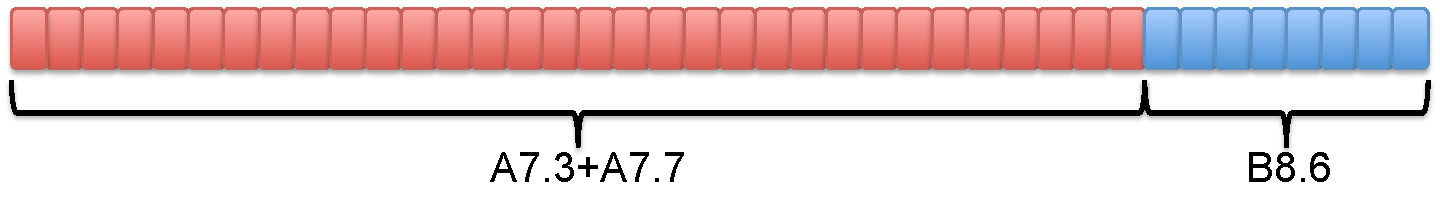
\includegraphics[scale=0.5]{figures/noto_cells.pdf}
\caption{\textbf{Notochord cells.}The primary notochord cell (blue) also known as the A-lineage are specified at the 64-cell stage. There are a total of 32 primary notochord cell that come from the A7.3 and A7.7 blastomere, and the intercalation of the cell happen in a semi-random stochastic manner.The secondary notochord cells (red) comes from the B8.6 blastomere and are specified at the 110-cell stage, one cell division after the primary notochord cells.}
\label{fig:noto_cells}
\end{figure}

Although a tailed larvae is typical of most ascidians, several species with in the Stolidobranchia order have individually undergone tail-loss, many of which fall in the Molgulidae \cite{berrill_studies_1931, jeffery_evolution_1999, huber_evolution_2000, maliska_molgula_2010}. The tail-less\textemdash anural\textemdash species develop in a similar manner and are indistinguishable from their tailed\textemdash urodele\textemdash counterparts up to late gastrulation \cite{berrill_studies_1931, swalla_interspecific_1990, jeffery_factors_1992}. Anural ascidians lack several urodele features including an intercalated and extended notochord, differentiated muscle cells and the otilith sensory organ. The absence of differentiated muscles cells and intercalated notochord are the cause for the lack of tail in these species \cite{miyamoto_formation_1985, swalla_interspecific_1990}. The development of several tail-less species have been studied. \textit{M. tectiformis} notochord cells do not divide again after the 10 precursor cells are formed and \textit{M. occulta} stops dividing after 20 cells \cite{jeffery_evolution_1999}. The same occurs in \textit{M. bleizi}, however after the 20 notochord cells are formed, the embryo attempts to make a tail but never completes the process \cite{swalla_novel_1993}. It has also been shown that chordate embryos without fully developed notochord and/or muscle cells do not fully elongate or fail completely to develop a tail \cite{jeffery_evolution_1999,takada_brachyury_2002,stemple_structure_2005}. 
Seeing that most ascidians have tailed larvae and that the tail can be restored through the use of interspecies hybrids, the lack of tail has been shown to be a loss of function. \textit{M. oculata} and \textit{M. occulta} both of the Roscovita clade have been shown to produce hybrids in lab conditions. Of the known \textit{Molgula} species \textit{M. occulta} and \textit{M. oculata} are the only two that can hybridize. Although \textit{M. occulta} and \textit{M. oculata} have been found to dwell in the same habitat, hybrids have not been found in nature and have only been produced in lab conditions. Fertilizing \textit{M. oculata} eggs with \textit{M. occulta} sperm in most cases produce embryos with fully formed tails. The reciprocal hybrid produces an embryo with 20 notochord cells like \textit{M. occulta}, however the notochord cells converge and extent like \textit{M. oculata} \cite{swalla_interspecific_1990}. The ascidian tail has been shown to form in the presence of notochord and the absence of muscles cells \cite{miyamoto_formation_1985} and the hybrid tail is not flaked by muscles as that of tail species \cite{swalla_novel_1993}. However, also it has been shown that embryos that develop urodele features are batch specific, and only in embryos that express the p58 which is associated with cytoskeleton are urodele features restored \cite{swalla_identification_1991,jeffery_factors_1992}. It has also been shown that in hybrid embryos in which urodele features were restored, the number of cells that express acetylcholinesterase (AChE) in a vestigial muscle cell lineage increased in comparison to hybrids lacking urodele features and \textit{M. occulta} \cite{jeffery_evolutionary_1991}. This along with evidence that with may have been, the ancestral notochord\textemdash the axochord\textemdash is muscle based \cite{lauri_development_2014}, shows strong evidence for the need of both notochord and muscles cells for the formation of the ascidian tail. 

\section{Brachyury has been shown to be the  }

\textit{Brachyury} a T-box transcription factor, has been identified to be essential for notochord development \cite{yasuo_conservation_1998}. The notochord induction is regulated by the \textit{FGF/MAPK/Ets} signaling cascade \cite{minokawa_binary_2001}. Where the A6.2 and A6.4 notochord/nerve cord precursors are induced by \textit{FGF9/16/20} at the 32-cell stage, just after the 7th cell cleavage \cite{satoh_ascidian_2001}. It was observed from isolation experiments that notochord/nerve cord precursors that loss \textit{FGF9/16/20} competence at the 32-cell stage assume the default nerve cord cell fate, the converse is true for presumptive nerve cord blastomeres that are introduce to \textit{FGF}, they forgo their default nerve cord fate and choose the notochord fate \cite{yasuo_conservation_1998,minokawa_binary_2001}. If \textit{FGF9/16/20} is not present at the 32 cell stage competence is lost, \textit{bra} is not induced and the notochord can no longer from \cite{nakatani_basic_1996,nakatani_duration_1999}. This is because \textit{MAPK} is not activated and the induction of \textit{bra} and repression of \textit{FoxB} are not carried out \cite{hashimoto_transcription_2011}. Without the repression of \textit{FoxB TF} the notochord cell fate is repressed through the repression of \textit{bra}. It has been observed in \textit{H. roretzi} that \textit{FoxB} represses the activation of \textit{bra} predominately through the binding of Fox BS1 (GCACTGA\textit{ACAAACA}TACATAG). \textit{FoxB} is activated by \textit{ZicN} and present in both nerve cord and notochords precursors, however is repressed by \textit{MAPK} in the notochord cell lineage at the 64-cell stage \cite{hashimoto_transcription_2011}. \textit{MAPK} is thought to be repressed by \textit{Ephin} which is one of the key differences between notochord and nerve cord determination. At this point \textit{bra} is expressed first weakly in the at the 64-cell stage in the notochord/nerve chord precursors \cite{yasuo_ascidian_1994} and unlike other chordates, in ascidians \textit{bra} is only expressed in the notochord cells \cite{yasuo_function_1993,corbo_characterization_1997,hotta_temporal_1999,takada_brachyury_2002}. Although \textit{bra} is necessary, its presence does not guarantee a tail. \textit{M. occulta} and \textit{M. tectiformis}, two tailless \textit{Molgula}, both express \textit{bra}. In both cases \textit{bra} expression stop earlier than that of \textit{M. oculata}, but produce different results. \textit{Bra} is expressed in the 10 precursor notochord cells in \textit{M. occulta}, another round of cell division occurs which does not in \textit{M. tectiformis}.  In these two species of \textit{Molgula} muscle actin became pseudo genes, however the mutation in the muscle actin genes are not the same \cite{swalla_novel_1993,jeffery_evolution_1999}. \textit{Manx} is another gene identified to be important for tell development in \textit{Molgula}, and is lowly expressed in \textit{M. occulta}, and has been shown to restore the hybrid tail \cite{swalla_requirement_1996, swalla_multigene_1999}. 
  
After cell specification, the notochord cells must converge, intercalate and extend. The Planar Cell Polarity (PCP) pathway is involved in cell movement during this process and mutations in \textit{prickle}\textemdash a known PCP gene\textemdash have shown to cause a shortened ascidian tail affecting both the mediolateral intercalation and the elongation of the ascidan tail \cite{jiang_ascidian_2005}. The \textit{pk} mutant \textit{aimless} produces a truncated tail, however the polarity of the nuclei are present, showing that prickle does not establish polarity with in the cell but polarity between cells, acting in a local manner and perhaps their is a global organizer \cite{jiang_ascidian_2005,kourakis_one-dimensional_2014}. However, even in the absence of the PCP pathway considerable convergence and elongation of the notochord was observed in Ciona, driven by a presumed boundary effects \cite{veeman_chongmague_2008}.

Many of the upstream genes and transcription factors that interact with \textit{bra} has been studied in fair detail, through known-outs, and cell isolation experiments. Not as much detail is known about the downstream genes regulated by \textit{bra}. On larger scale subtractive screening was done to identify genes downstream of \textit{bra}, 39 genes were initially found \cite{hotta_temporal_1999}. An attempt to characterize a number of these genes have been made, identifying functions such as extracellular matrix components (\textit{cadherin 8, entactin, fibronectin, laminin $alpha$1, $alpha$4, and $beta$1, and thrombospondin}, genes involved in cell shape and polarity (\textit{pk, trop, ERM, ACL}), axon guidance (\textit{netrin, semaphorin 3A}), amongst a host of other biological processes \cite{hotta_characterization_2000,hotta_brachyury-downstream_2007,kugler_evolutionary_2008}. 

\textit{Oikopleura} which are in the same subphyla\textemdash tunicates or urochordates\textemdash also develops in a typical chordate manner with a notochord and has a compact genome, however, in Larvacean there are 20 notochord cells \cite{seo_miniature_2001,denoeud_plasticity_2010}. \textit{Oikopleura} retains its tail during its adult life stage and at this point \textit{bra} is not expressed in the adult notochord, however, \textit{bra} is expressed in the same manner in the developing larval notochord as ascidians \cite{bassham_brachyury_2000,nishida_development_2008}. When comparing gene networks, \textit{Oikopleura} did not exhibit the same mechanism for tail development as \textit{Ciona}, of the 50 bra target genes previously identified cite only 26 of them had orthologs, almost 50\% of the genes were not present \cite{kugler_evolutionary_2011}. Of the genes that did show homology, expression ranged from notochord specific to tail including possible notochord, to tissues that were clearly not the notochord.


\section{Assembling and analyzing data}
One of the major advances in science in the past 20 years was the implementation of sequencing technologies. These technologies allowed us to examine problems in ways not previously possible. The first wave was Sanger sequencing in the 1986, but was not broadly used until 10 years later. Another technology, mircoarrays, which became popular starting in the mid '90s, allow us to look at a wide spectrum of genes and understand relative expression within a sample. Kobayashi et al. \cite{kobayashi_differential_2013} isolated and analyzed gene expression in notochord (A7.3+A7.7) and nerve cord (A7.4+A7.8) precursors using microarrays. This study was able to identify 106 genes expressed in the notochord precursor and 68 expressed in the nerve cord precursor at the 64-cell stage. Of these the genes, 36 notochord genes and 25 nerve chord genes were confirmed via Whole Mount In Situ Hybridization in the respective cells. This demonstrates the power of this technique, however, prior knowledge is needed. \textit{C. intestinalis} was sequenced using sanger sequencing, and is well assembled and most well annotated \cite{dehal_draft_2002}. In addition to long reads (Sanger) scaffolding was done using experimental data\cite{satou_improved_2008}. Sanger sequencing able to sequence whole genomes without the need of prior knowledge to identify novel genes but is costly and time consuming\cite{metzker_emerging_2005,liu_comparison_2012}. 

Sanger was the $1$\textsuperscript{st} generation of sequencing technologies, and currently both $2$\textsuperscript{nd} and $3$\textsuperscript{rd} generation are in use, with Roche 454, Ion Torrent, Illumina and PacBio are the most wide spread. These technologies are far easier to produce data and much less costly than sanger sequencing \cite{metzker_emerging_2005}. There are many trade-offs for each of the technologies, cost per MB, sequencing time, prep cost, error rate and sequencing bias; 454 and PacBio have longer reads than Illumina and Ion Torrent, 800 bp and 1+kbp, respectively. However, both Illumina and Ion Torrent's short reads are cheaper to generate, produce more reads and better for counting, in addition to PacBio having a high error rate \cite{glenn_field_2011}. Illumina and Ion Torrent have the best error rates and while Ion Torrent calls more more Single nucleotide polymorphisms, it also calls more false positives.  For this reason, amongst other Illumina is the most used because it is the most versatile and preforms the best in general \cite{quail_tale_2012}. This drop in price and produced many of the assembled genomes within the Tuncata phyla. Outside of this project there are eight tunicate genomes assembled; \textit{C. intestinalis}, \textit{C. savignyi}, \textit{Oikopleura dioica}, \textit{Botryllus schlosseri}, \textit{Halocynthia uranium}, \textit{H. foretzi}, \textit{Phallusia fumigata}, and \textit{P. mammilata}, but no \textit{Molgula} genomes. 

\chapter{Evaluating a lightweight transcriptome assembly pipeline on two closely related ascidian species}



\section{Introduction}

Next generation sequencing (NGS) has allowed us to study organisms with a broader lens, looking at entire genomes and transcriptomes instead of single genes.  This capability is particularly important for non-model organisms where little prior knowledge may be available, and where NGS readily enables whole-transcriptome analyses \citep{wang_rna-seq:_2009}, allowing us to study organisms that are ecologically or evolutionarily interesting.

There are now several sequencing technologies, Illumina being one of the most versatile \citep{glenn_field_2011}, that can produce millions of short reads ranging from 75 to 150 bp in length at a low cost \citep{zhang_impact_2011}. As sequencing costs continue to drop, transcriptomes from multiple developmental stages of non-model organisms can easily be sequenced. Various types of \textit{de novo} assembly algorithms and reference based assembly approaches have been developed to handle this massive influx of transcriptomic data \citep{pop_genome_2009,vinson_assembly_2005,stapley_adaptation_2010}. It has been shown in some cases that mapping mRNA-seq reads to a reference genome yields better transcriptomes than \textit{de novo} assemblies, even if the genome is 5-15\% divergent \citep{vijay_challenges_2012}. However, with many non-model organisms, no nearby reference genome is available.

\textit{De novo} transcriptome assembly is the only solution for organisms with no evolutionarily close reference genome.  Transcriptome assemblers such as Trinity \citep{grabherr_full-length_2011} and Velvet/Oases \citep{zerbino_velvet:_2008,schulz_oases:_2012} use De Bruijn-graph based \textit{de novo} approaches which build graphs connecting the reads based on k-mer overlap. These graphs are then traversed via an Eulerian path algorithm to assemble transcripts. Because De Bruijn graphs are based on exact matches between DNA words, increasing numbers of sequencing errors result in an exponential number of new paths, adding to the complexity of the graph and, in turn, increasing the assembly time and memory requirements \citep{pop_genome_2009}.

Here we have sequenced the transcriptomes of several developmental stages of \textit{Molgula occulta} and \textit{Molgula oculata}\textemdash two closely related, free-spawning ascidian species, with no available reference genome. \textit{Ciona intestinalis} and \textit{Ciona savignyi} are the closest related ascidian species with well-assembled genomes, but are not close enough to use as a nucleotide reference for transcriptome construction. In this paper, we describe an efficient, easy to follow protocol for the transcriptome assembly of two Molgulid developmental transcriptomes. A crucial part of this protocol is the use of a preprocessing step that normalizes read abundances prior to assembly, called ``digital normalization.'' We study the effect of digital normalization on assemblies performed with both Trinity and Velvet/Oases.  We compare our approach to the results of running Trinity and Velvet/Oases without digitally normalized reads and show that our approach recovers essentially the same gene content but has significantly reduced requirements for time and memory.  This reduction in time and memory lets us assemble transcriptomes efficiently using cloud resources, making our results exceptionally easy to reproduce \citep{haas_novo_2013}, and more broadly enabling transcriptome assembly by researchers without access to large computer resources.

\section{Methods}
\subsection{Sequencing preparation}
\textit{M. occulta} and \textit{M. oculata} were collected by dredging off the shores of Roscoff, France near La Station Biologique. Swalla et al have previously described the maintenance \citep{swalla_interspecific_1990} and culturing \citep{swalla_multigene_1999} of the animals. The transcriptomes of \textit{M. occulta} and \textit{M. oculata} were sequenced at Michigan State University (MSU) in the Research Technology Support Facility on Illumina HiSeq 2000. Five lanes of sequences were generated for \textit{M. occulta}, two lanes of the gastrula stage (F+3), one of neurula (F+4), one of early tailbud (F+5), and one from the tailbud (F+6) stage (Table 1). Three lanes of sequences were generated for \textit{M. oculata}, one each for the gastrula, neurula and tailbud stage. 10$\mu$g of RNA were sequenced for each stage with the exception of \textit{M. occulta} F+4, where 1.05$\mu$g of RNA was sequenced. On average each embryonic stage yielded 48 million reads of 75 base pairs (bp) in length with paired-end insert lengths of 250 bp. All reads can be found in the NCBI short read archive (SRA) under accession number SRP040134. 

\subsection{Assembly protocol}
Below is an overview of the steps used for the \textit{de novo} assembly and annotation of our transcriptomes.
\begin{enumerate}
	\item Quality trimming and filtering of raw reads.
	\item Apply digital normalization to decrease data size.
	\item Assemble transcriptome.
	\item Assess transcriptome quality.
	\item BLAST (gene recovery/identification).
\end{enumerate}
Scripts used to run these steps can be found in the following GitHub repository: https://github.com/ged-lab/2014-mrnaseq-cloud
\subsection{Pre-assembly read trimming and normalization} 
Low quality bases were trimmed and low quality reads were removed using quality-trim-pe.py found in the scripts directory of the repository. A hard trim is done at a Phred quality score of 33 and reads less than 30 base pairs in length are discarded. This process creates a paired and singleton fastq file for each library because of the removal of low quality reads. The filtering of reads allows for better assembly and better mapping, although it may also reduce sensitivity to low-expressed transcripts \citep{lohse_robina:_2012, macmanes_optimal_2014}. The reads were initially 75 bp long, and the average base pair (bp) length was 63 bp after quality trimming and filtering. After quality trimming reads were either directly assembled, or first preprocessed with digital normalization and then assembled. 

Digital normalization (diginorm) is a technique that down samples reads from highly abundant transcripts while retaining approximately the full sequence information content of the reads \citep{brown_reference-free_2012}. Here, for each species, reads from all stages were normalized together to build a common reference transcriptome; reads were normalized to a k-mer coverage of 20 with the k-mer size set to 20 as well.  The initial data set from \textit{M. occulta} contained 237 million reads from 5 lanes, and \textit{M. oculata} contained 150 million total reads; after digital normalization, the \textit{M. occulta} dataset was reduced to 91.6 million reads and \textit{M. oculata} was reduced to 50 million reads, a ~60\% and ~77\% reduction respectively (Table~\ref{fig:time_and_memory.pdf}).

\begin{table}[ht]
\centering
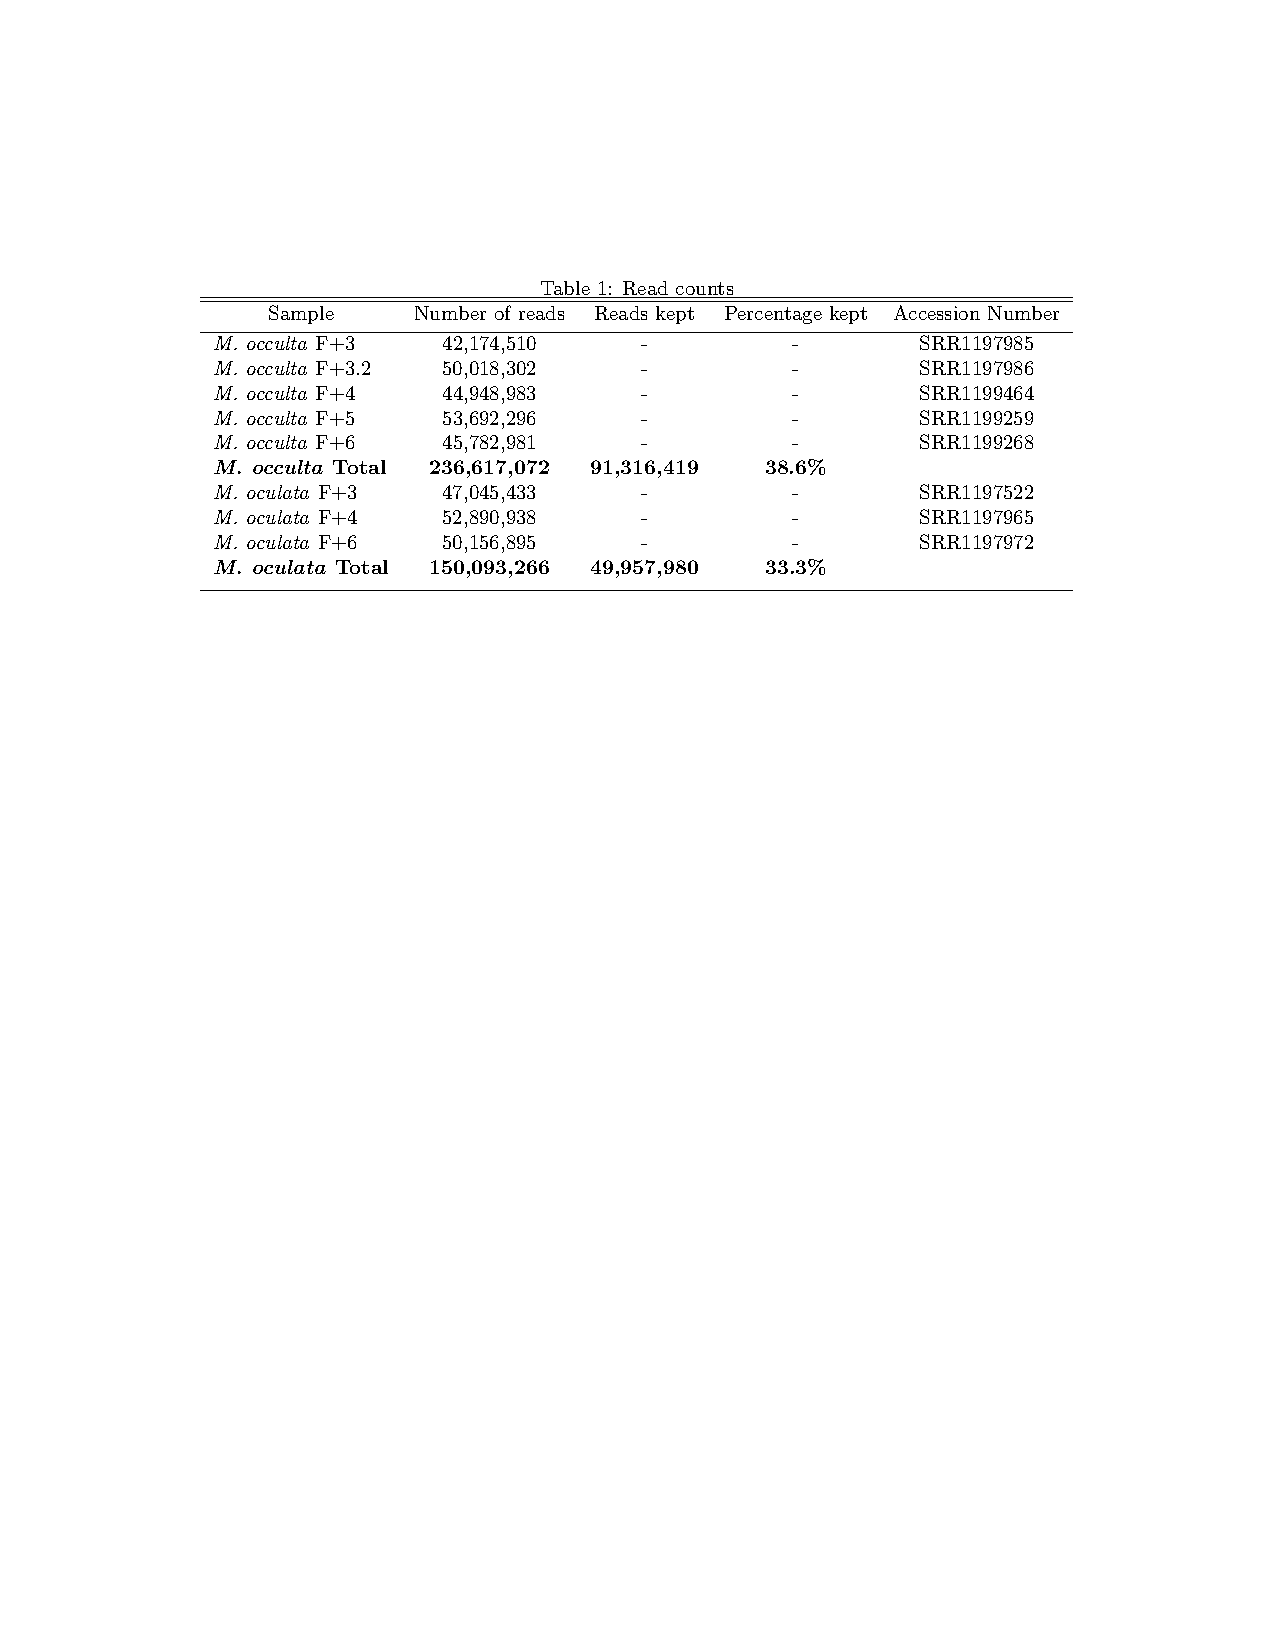
\includegraphics[scale=1.0]{manuscript/Table1.pdf}
\caption{\textbf{Digitally normalized reads.} The number of reads sequenced before and after digital normalization are shown for each lane of sequencing. The percentage of total reads kept after digital normalization is shown in bold. \textit{M. occulta} had approximately \mytilde237 million reads and was reduced to 91 million reads, a 60\% reduction. \textit{M. oculata} had 150 million reads and reduced by 77\% to \mytilde50 million reads. }
\label{fig:Table1.pdf}
\end{table}

\subsection{Transcriptome assembly}
We used the Trinity (r20140413p1) and Velvet/Oases (v1.2.08/v0.2.08) assembler packages, both of which have performed well on other data sets \citep{vijay_challenges_2012,grabherr_full-length_2011,schulz_oases:_2012}.  Velvet was initially developed to assemble genomes, and the Oases add-on package was developed for transcriptome assembly, since transcriptomes have variable coverage and many isoforms.  Since Oases cannot be run without Velvet, we refer below to transcriptomes assembled with Velvet and Oases as Oases assemblies. Unlike Trinity, Oases requires the choice of a k-mer overlap for assembly; we chose several k values ranging from k = 21 to k = 35, for odd values of k, with scaffolding turned off. After assembly, the Oases transcriptomes with the highest number of blast hits to \textit{C. intestinalis} were selected for further analysis. The Trinity assembler was run with default parameters.

All assemblies were performed on the Michigan State University (MSU) High Performance computing cluster (HPCC).  All diginorm assemblies were repeated on Amazon EC2 machines as a proof of concept.
After assembly, transcripts shorter than 200 bp in length were removed, and CD-HIT was used to eliminate small transcripts with 99\% identity to longer transcripts using the following command: ``cd-hit-est -i \textless transcript file\textgreater -c 0.99 -o \textless output file\textgreater'' \citep{li_cd-hit:_2006}.

To choose the best k-mer parameter for the Oases assemblies, \textit{C. intestinalis} proteins were searched with TBLASTN (e-value cutoff of 1e-6) against each Oases assembly and the transcriptome with the most hits was selected for further analysis.
\subsection{Gene identification}
We used standalone BLAST to find reciprocal best hits (RBH) between the eight assembled transcriptomes and the \textit{C. intestinalis} proteome retrieved from NCBI under search term ``(ciona intestinalis) AND Ciona intestinalis [porgn:\_\_txid7719]''. At the time of retrieval there were 16,123 sequences and they were downloaded and stored in the GitHub repository under the file name ``ciona\_transcriptome.fa'' in case the sequences change on NCBI. An e-value cutoff of 1e-6 was used as a minimum threshold for transcript identity.  The find-reciprocal-2.py script was used to identify the RBH.
\subsection{Read mapping}
	To determine the inclusion of reads in the various transcriptome assemblies trimmed reads were mapped to their respective species using bowtie2 v2.2.1 \citep{langmead_fast_2012}. For both unnormalized read and diginorm assemblies the full set of trimmed reads were used for mapping. Default parameters were used, and both paired ends and singletons were mapped. Samtools v0.1.19 \citep{li_sequence_2009} was used for format conversion from SAM to BAM format, and also to calculate the percentage of mapped reads. The BAM files were also used to calculate the coverage of transcripts.

\section{Results}

\subsection{Digital normalization reduces the resources needed for assembly}
 The \textit{M. oculata} unnormalized read data set assembled with Oases used 44 CPU hours and 85 GB of RAM. The Oases assembly done with the digitally normalized reads took \mytilde22 CPU hours and 21 GB of RAM (Figure~\ref{fig:time_and_memory.pdf}); this includes the time and memory required to run the digital normalization pipeline. \textit{M. occulta} diginorm Oases assembly required over 100 GB of RAM, and the raw read Oases used 300 GB of RAM. The raw read Oases assemblies for both species took twice as long and needed at least three times as much memory when compared to the diginorm reads.

The difference in assembly time and memory between diginorm and raw reads was not as large when using the Trinity assembler. Diginorm completed its assemblies several hours faster than assembling raw reads, \mytilde15 hours compared to \mytilde26 hours for \textit{M. oculata} and \mytilde24 hours compared to \mytilde39 hours for \textit{M. occulta}. \textit{M. oculata} unnormalized reads did not require much more memory than the normalized reads\textemdash 16.8 GB and 15.65 GB, respectively. Diginorm had a larger effect on \textit{M. occulta}, assembling \textit{M. occulta} normalized reads with 23.17 GB of RAM versus 34.14 GB of RAM for the unnormalized reads (Figure~\ref{fig:time_and_memory.pdf}).

\begin{figure}[tbp]
\centering
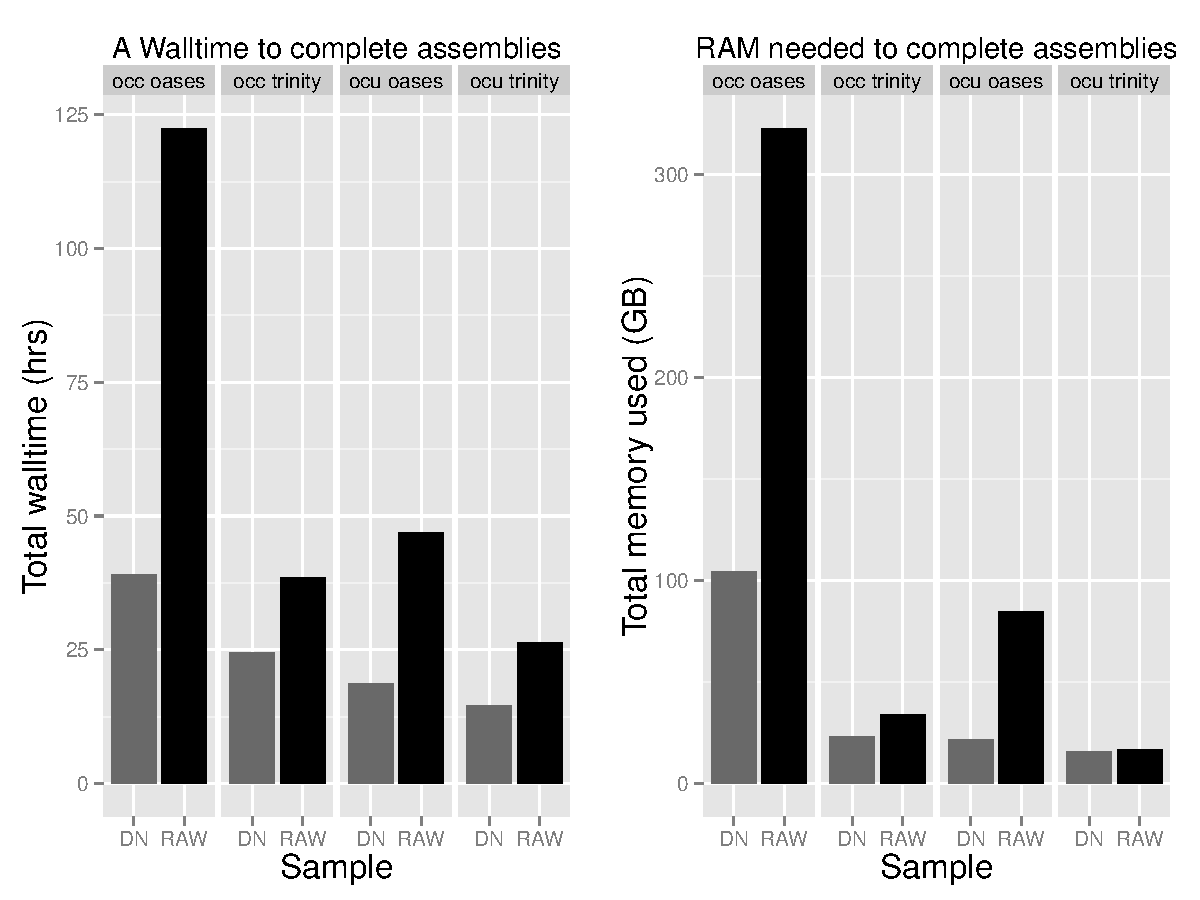
\includegraphics[scale=0.5]{manuscript/figure_1_time_and_memory.pdf}
\caption{\textbf{Wall time and memory requirements for assemblies.} Wall time (left) in hours to complete the diginorm (DN) and raw read (RAW) assemblies for both species and assemblers. Oases assembled multiple k's, 21 $\leq$ k $\leq$ 35 opposed to Trinity that uses only a single k. This is one reason the assembly times differed. (right) Shows the memory used to assemble each of the transcriptomes. M. oculata (ocu) transcriptomes assemble in less time than M. occulta (occ) because they have fewer lanes of reads to assemble. In all cases diginorm required less time and memory to complete the assembly.}
\label{fig:time_and_memory.pdf}
\end{figure}
  
\subsection{Assembly statistics varied by preprocessing approach and assembler}
Oases run with the diginormed reads yielded fewer total transcripts than Oases run with the unnormalized reads. The \textit{M. oculata} diginorm assembly produced 300 fewer transcripts, and the \textit{M. occulta} diginorm assembly produced 227 fewer transcripts (Table~\ref{fig:Table2.pdf}). Digital normalization had the opposite affect when using Trinity for assembly, increasing the total number of assembled transcripts by 7,840 for \textit{M. oculata} and 9,197 for \textit{M. occulta}.

\begin{table}[tbp]
\centering
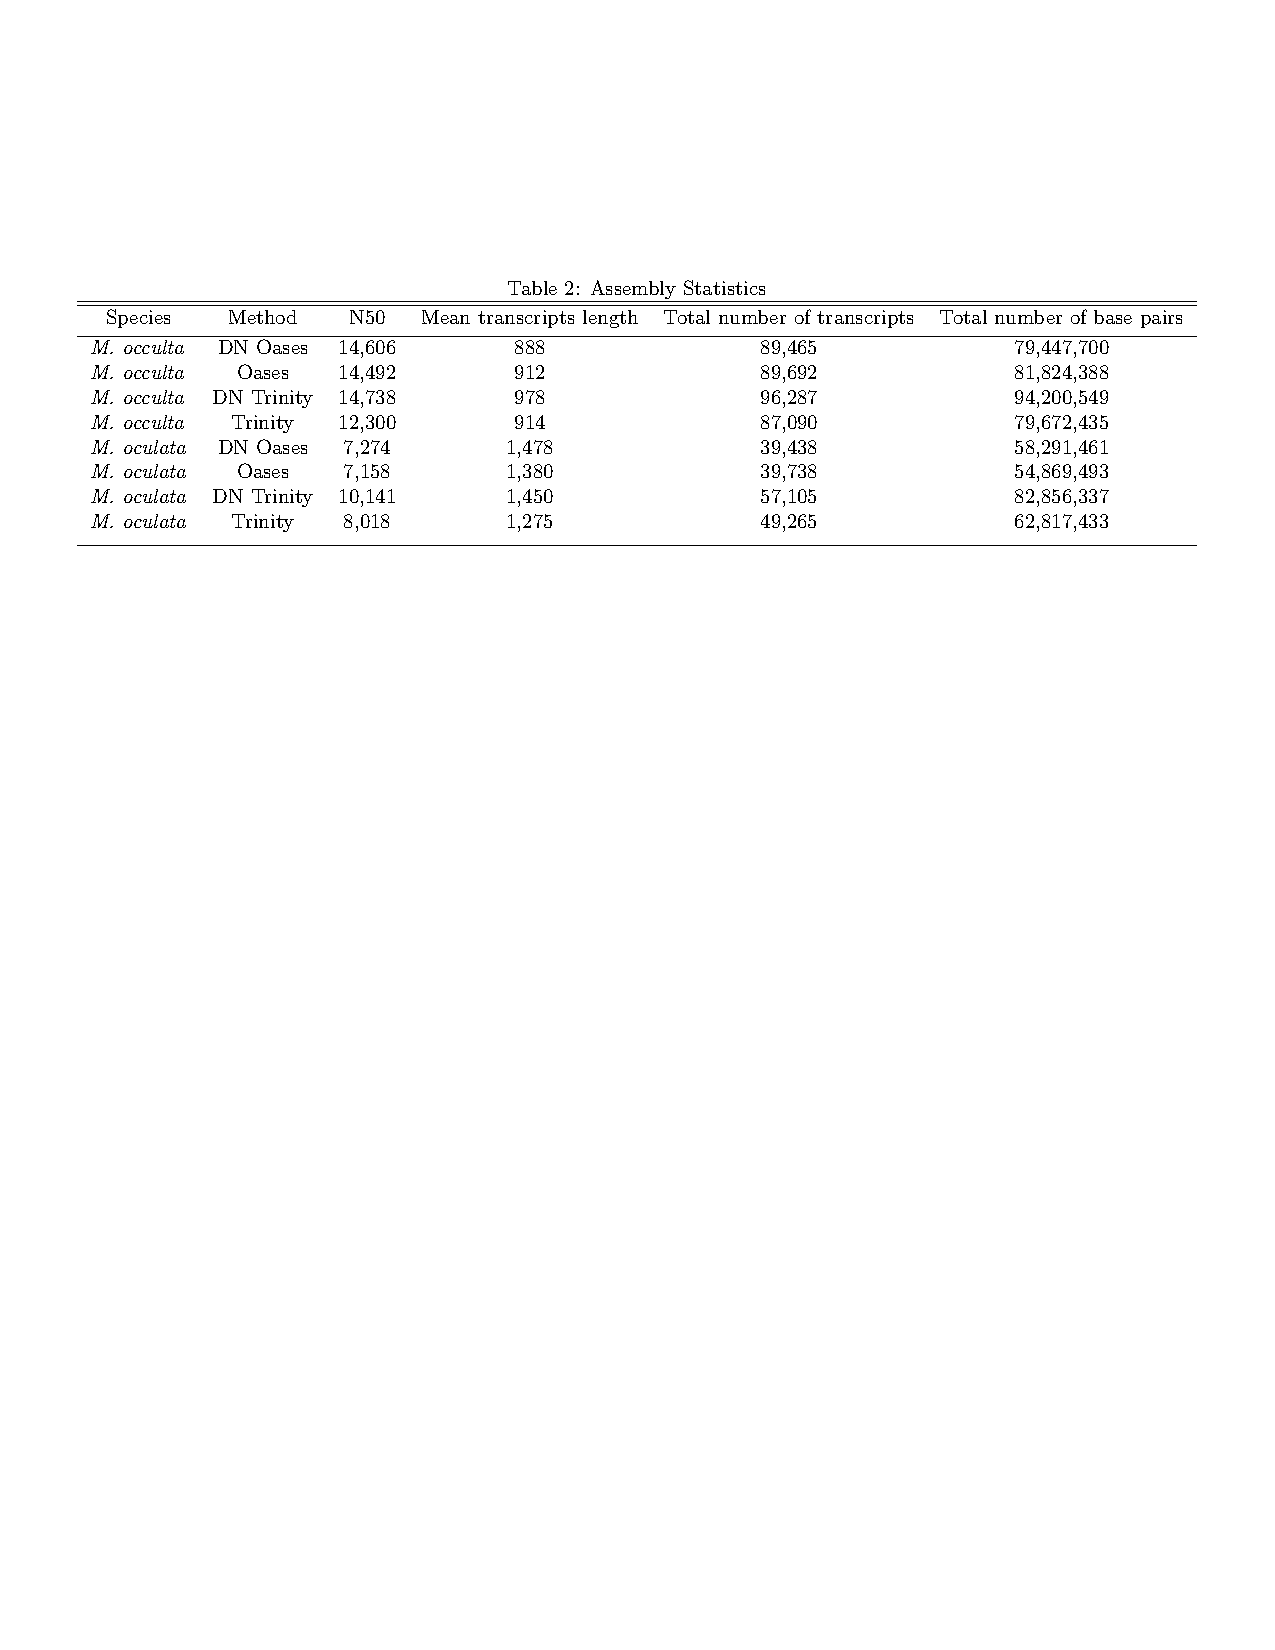
\includegraphics[width=\linewidth]{manuscript/Table2.pdf}
\caption{\textbf{Transcriptome metrics.} Several metrics used to assess the assembled transcriptomes. The N50, mean transcript length, total number of transcripts and total number of base pairs are listed for each transcriptomes.}
\label{fig:Table2.pdf}
\end{table}
   
Trinity produces 6.8k (7.6\%) more transcripts than Oases for \textit{M. occulta} using the digitally normalized reads, and a 2.6k (2.9\%) decrease in the number of transcripts using the unnormalized reads. Trinity assembled more transcripts for both \textit{M. oculata} assemblies, a 17.6k (44.8\%) increase for diginorm and a 9.5k (24\%) increase for the raw reads. 

\subsection{Trinity assemblies include more low-abundance k-mers than Oases assemblies}
We next examined the k-mer spectrum of the assembled transcripts using k-mer abundances from the digitally normalized reads. The k-mer spectrum is an account of the information content of the reads and can be used to evaluate the ability of the assemblers to recover low-abundance transcripts \citep{pop_genome_2009}.  We first used digital normalization to reduce the reads to a median k-mer coverage of 20, so that the k-mer frequency spectrum peaked at a coverage of 20, and then plotted a cumulative abundance plot of those k-mers shared between the normalized reads and the assemblies. The results, displayed in Figure 2, show that Trinity recovers more low-abundance k-mers.  Also note that between assemblies done with the same assemblers, the k-mer distributions were very similar, suggesting that the k-mer spectrum is reflective of the underlying graph traversal algorithm used by the assembler. In addition the Trinity assemblies included more unique k-mers (Figure~\ref{fig:multiplicity})

\begin{figure}[!ht]
	\subfloat[\textit{M. occulta}\label{subfig-1:figure_2_Mocc_dist}]{%
	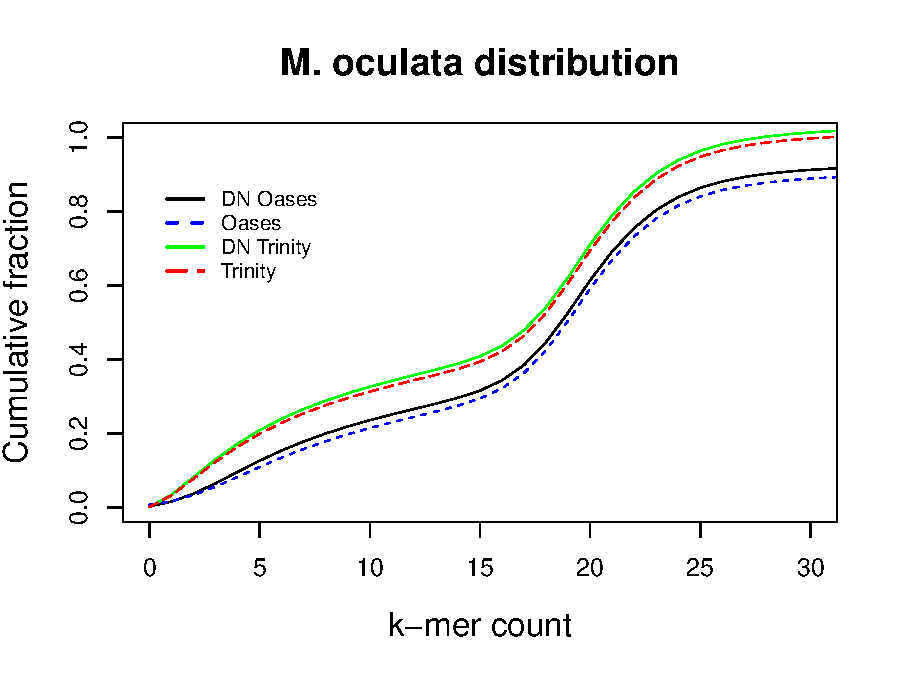
\includegraphics[width=0.45\textwidth]{manuscript/figure_2_Mocu_dist.pdf}
	}
	\hfill
	\subfloat[\textit{M. oculata}\label{subfig-2:figure_2_Mocu_dist}]{%
	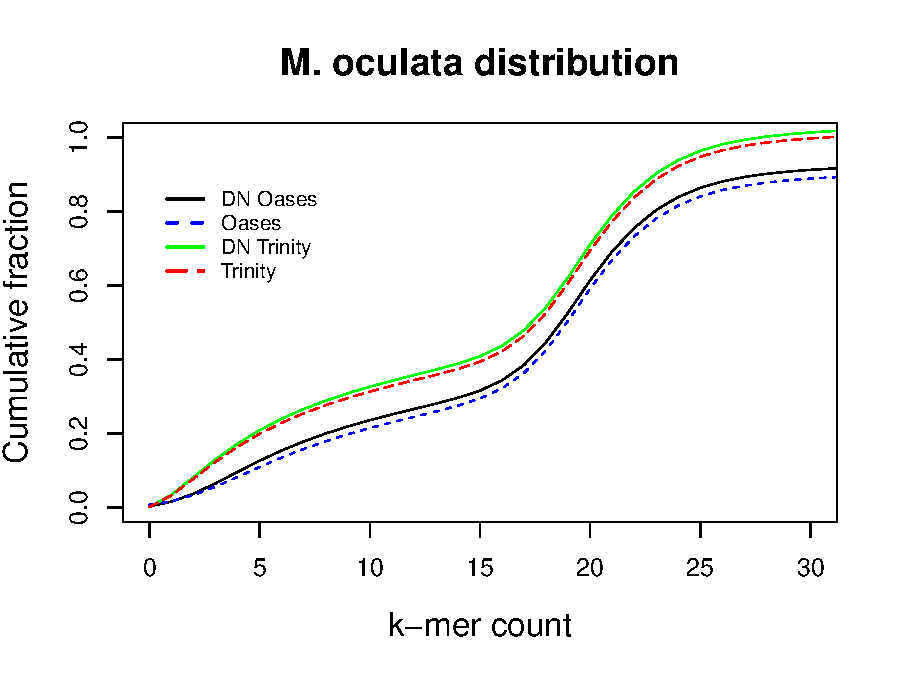
\includegraphics[width=0.45\textwidth]{manuscript/figure_2_Mocu_dist.pdf}
	}
	\caption{\textbf{K-mer distribution.} The k-mer distribution is shown for each assembler and assembly condition, diginorm (DN) and unnormalized reads. The k-mer distribution is the coverage of a given k-mer verses how many k-mers of that coverage is incorporated in the respective assemblies. Both Oases and Trinity assemblies are shown for ~\ref{fig:figure_2_Mocc_dist} \textit{M. occulta} k-mer distribution and  ~\ref{fig:figure_2_Mocu_dist} \textit{M. oculata} k-mer distributions. Trinity had a higher k-mer distribution for both species, reflective of the inclusion of more low abundance reads into the Trinity assemblies.}
	\label{fig:k-mer_spec}
\end{figure}

\begin{table}[tbp]
\centering
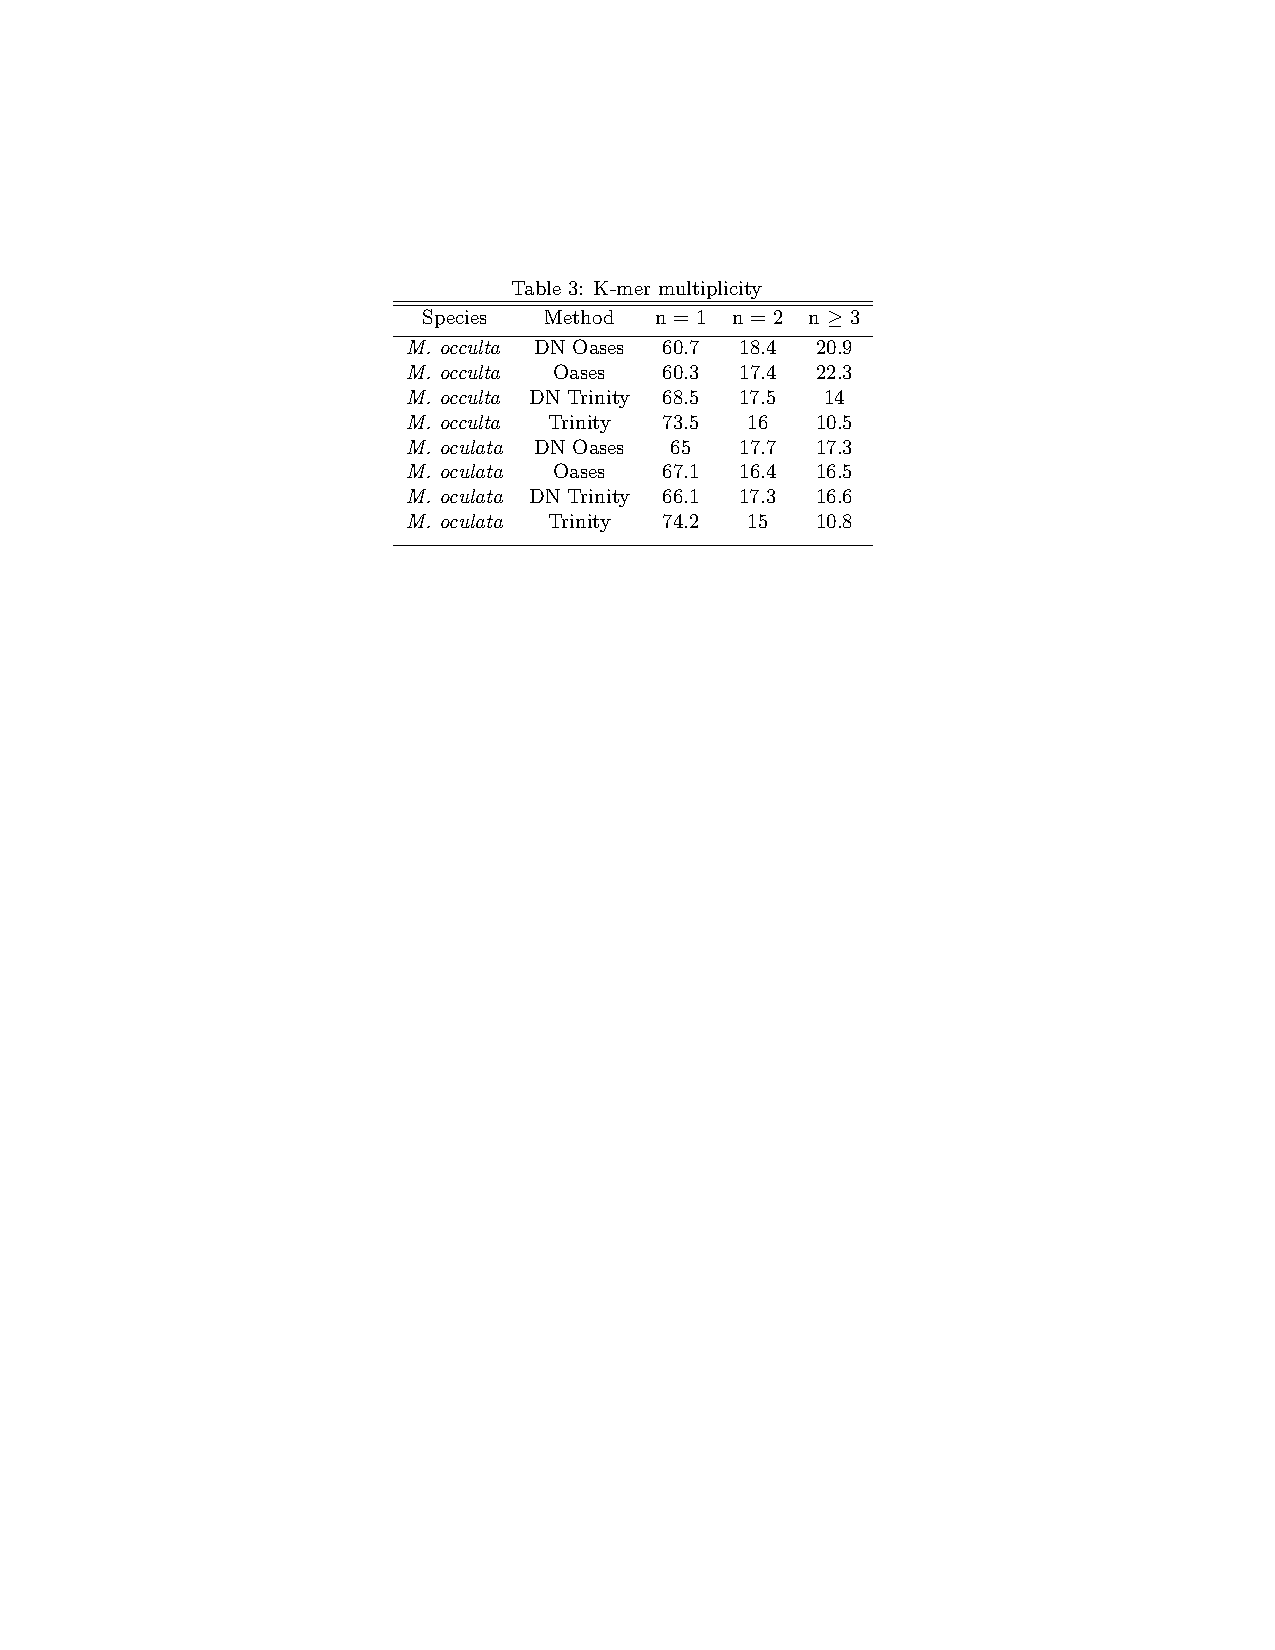
\includegraphics[width=0.4\linewidth]{manuscript/Table_3_multiplicity.pdf}
\caption{\textbf{Multiplicity.} The k-mer multiplicity shows uniqueness of each assembly. All k-mers with a multiplicity of one are unique. Trinity has a higher percentage of unique k-mers when comparing assemblers. The unnormalized Trinity had the highest number of unique k-mers overall.}
\label{fig:multiplicity}
\end{table}

\subsection{Read mapping shows high inclusion of reads in the assembled transcriptomes}
	We mapped the quality-filtered reads to the assembled transcriptomes to evaluate their inclusiveness. The F+3 stage of reads from \textit{M. occulta} had the lowest percentage of mapped reads, with the Oases unnormalized assembly mapping only 49\% of the reads, and the Trinity unnormalized assembly mapping 67\% (Figure 3\ref{fig:figure_3_mocc_mapping}). This was an isolated case: all other Oases assemblies contained at least 75\% of the reads for each time point and the Trinity assemblies contained at least 93\% of the reads for each time point. Trinity raw read assemblies tended to contain slightly more reads than the diginorm assemblies, while the opposite was true for Oases; however, in no case did the raw-reads assembly differ from the diginorm assemblies in more than 3\% of their read content.
\setcounter{subfigure}{0}
\begin{figure}[tbp]
	\begin{center}
	\subfigure[]{%
                \label{fig:figure_3_mocc_mapping}
                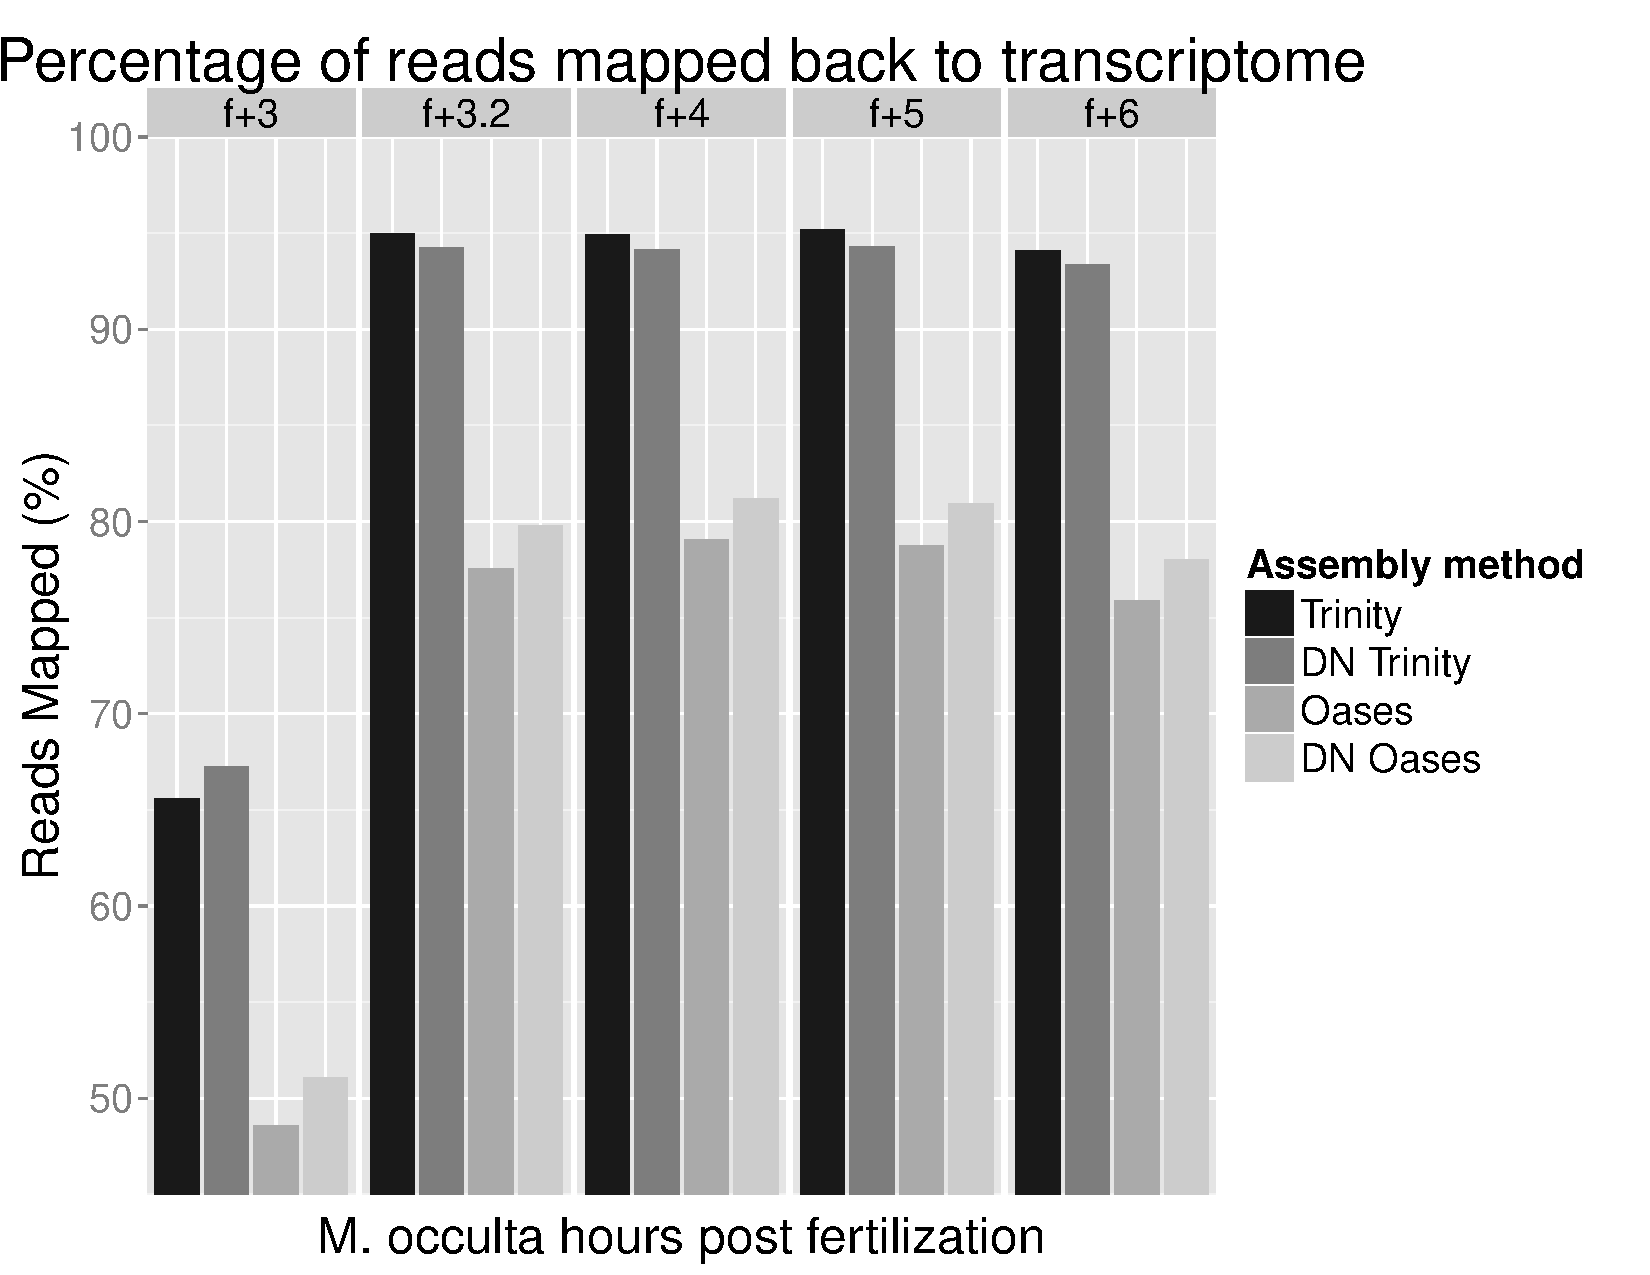
\includegraphics[width=0.4\textwidth]{manuscript/figure_3_mocc_mapping.pdf}
	}%
	\subfigure[]{%
                \label{fig:figure_3_mocu_mapping}
                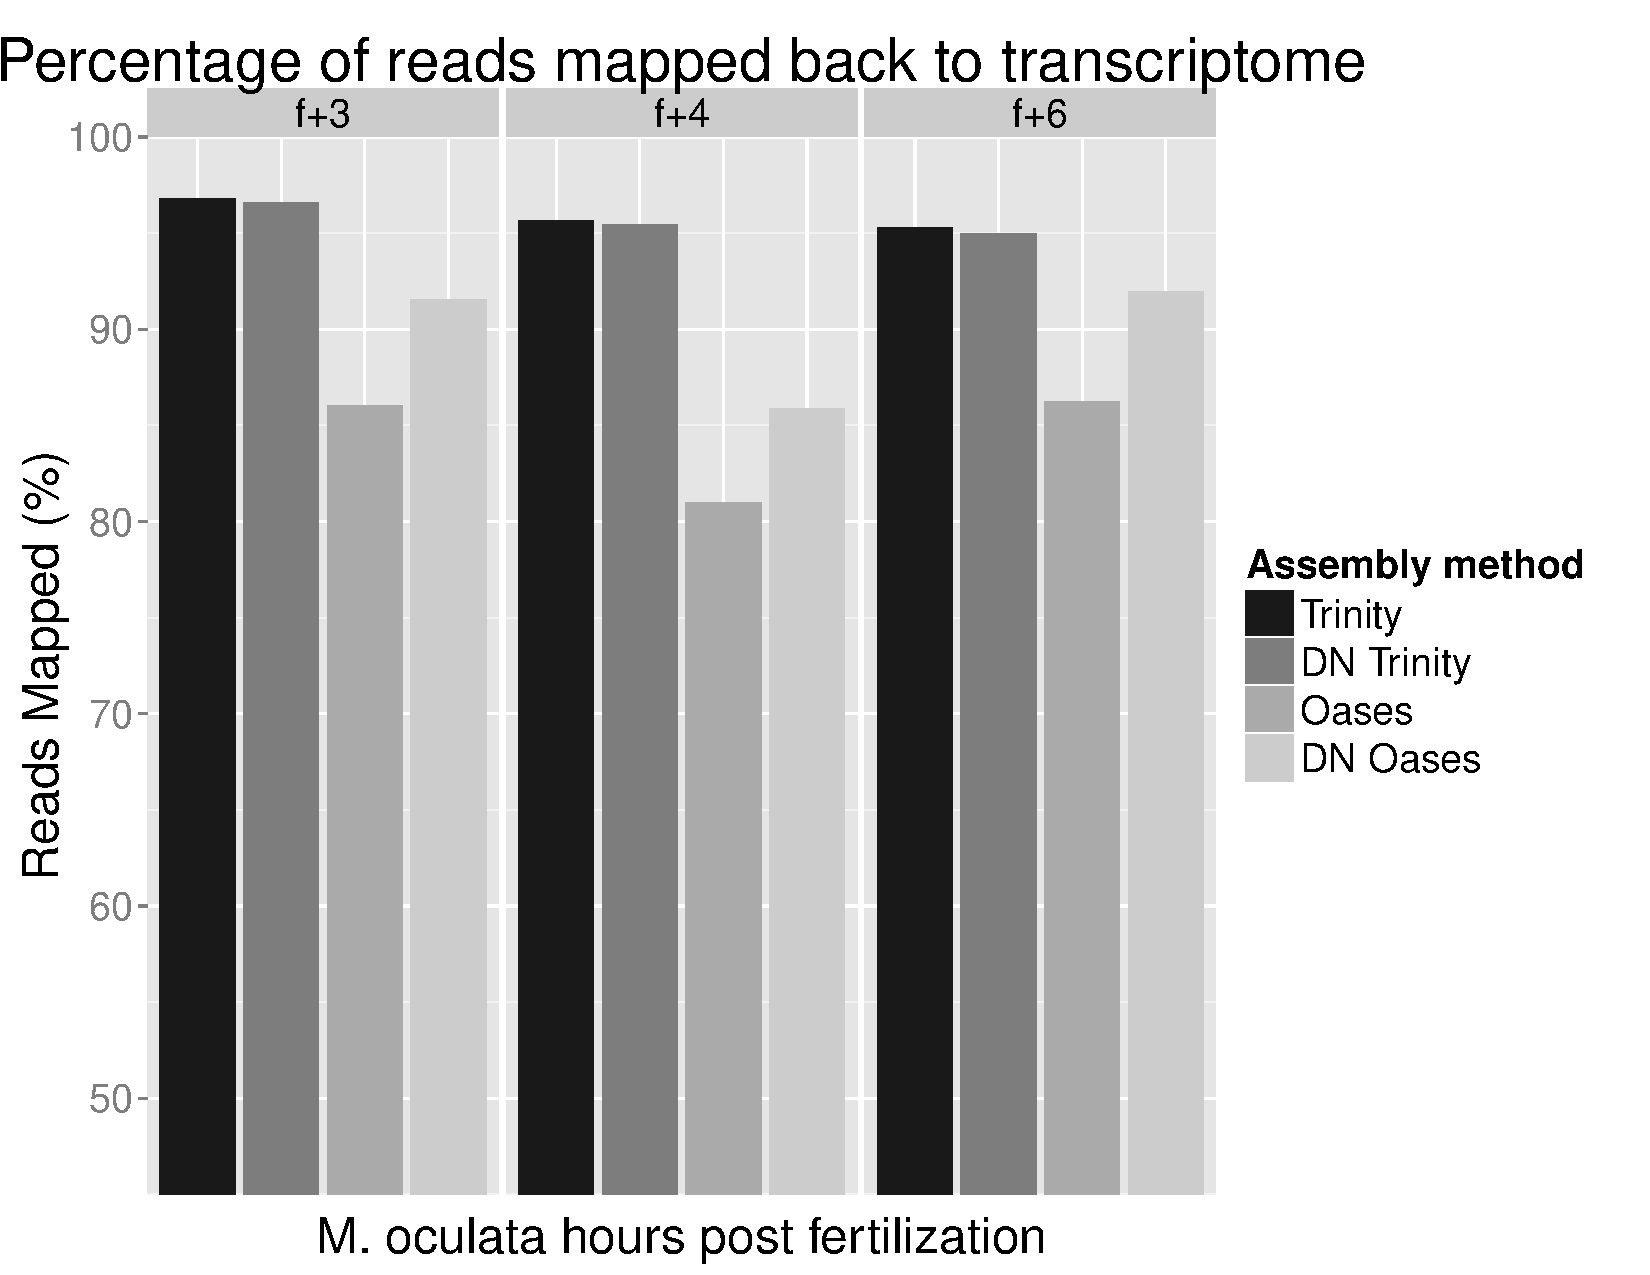
\includegraphics[width=0.4\textwidth]{manuscript/figure_3_mocu_mapping.pdf}
	}%
	\end{center}
	\caption{\textbf{Read mapping.} Unnormalized reads were mapped back to each of the assemblies to determine the inclusion of reads in the assembly. ~\ref{fig:figure_3_mocc_mapping}\textit{M. occulta} first round of gastrulation reads (f+3), showed the lowest mapping quality for all assemblies, with the lowest being raw Oases at 48.57\%. \textit{M. occulta} f+3 is the only case were mapping is less than 74\% and the only case where DN Trinity mapped more reads than Raw Trinity. ~\ref{fig:figure_3_mocu_mapping}\textit{M. oculata} unnormalized Oases performed the worst, with Trinity assemble having the best mappings. Trinity assemblies have more mapped reads than Oases for all conditions, with at least 93\% read mapping for both species. Raw Trinity typically mapped slightly more reads than DN, and the opposite occurs for Oases, with DN having more reads mapped to its assembly.  Note that the Y axis starts at 45\%.}
	\label{fig:read_mapping}
\end{figure}

\subsection{All assemblies recovered transcripts with high accuracy but varied completeness}
mRNAseq assembly accuracy can be calculated based on known transcripts generated from longer reads or reference genomes \citep{vijay_challenges_2012,martin_next-generation_2011}. We use Molgulid nucleotide sequences from NCBI to measure accuracy, and we define accuracy as the average BLAST identity score for the best match for each gene recovered \citep{li_sequence_2009}. There are 178 sequences from within the Molgula clade in the NCBI database. With the exception of \textit{M. occulta} unnormalized Oases assembly, all assemblies have hits to at least 113 out of these Molgula sequences (Figure 4). The Trinity assemblies for both species have hits to all 178 sequences. Oases assemblies have hits for more sequences using digital normalized reads, two additional hits for \textit{M. oculata} and 40 additional hits for \textit{M. occulta}. \textit{M. oculata} assemblies hits have high average accuracy in the 90 and 99 percentile for Oases and Trinity, respectively. Completeness is the percentage of a gene, transcript or protein that is recovered. Within the \textit{M. oculata} assemblies, the unnormalized Oases assembly has the lowest average completeness at 36\%, the Trinity assemblies round out at 60\% and the digital normalized Oases assembly has the highest average completeness at 72\%.  (Note that many of the \textit{Molgula} sequences are genomic, not coding, so we would not expect high completeness.)

\setcounter{subfigure}{0}
\begin{figure}[tbp]
	\begin{center}
	\subfigure[]{%
                \label{fig:figure_4_moccVsknownmolg}
                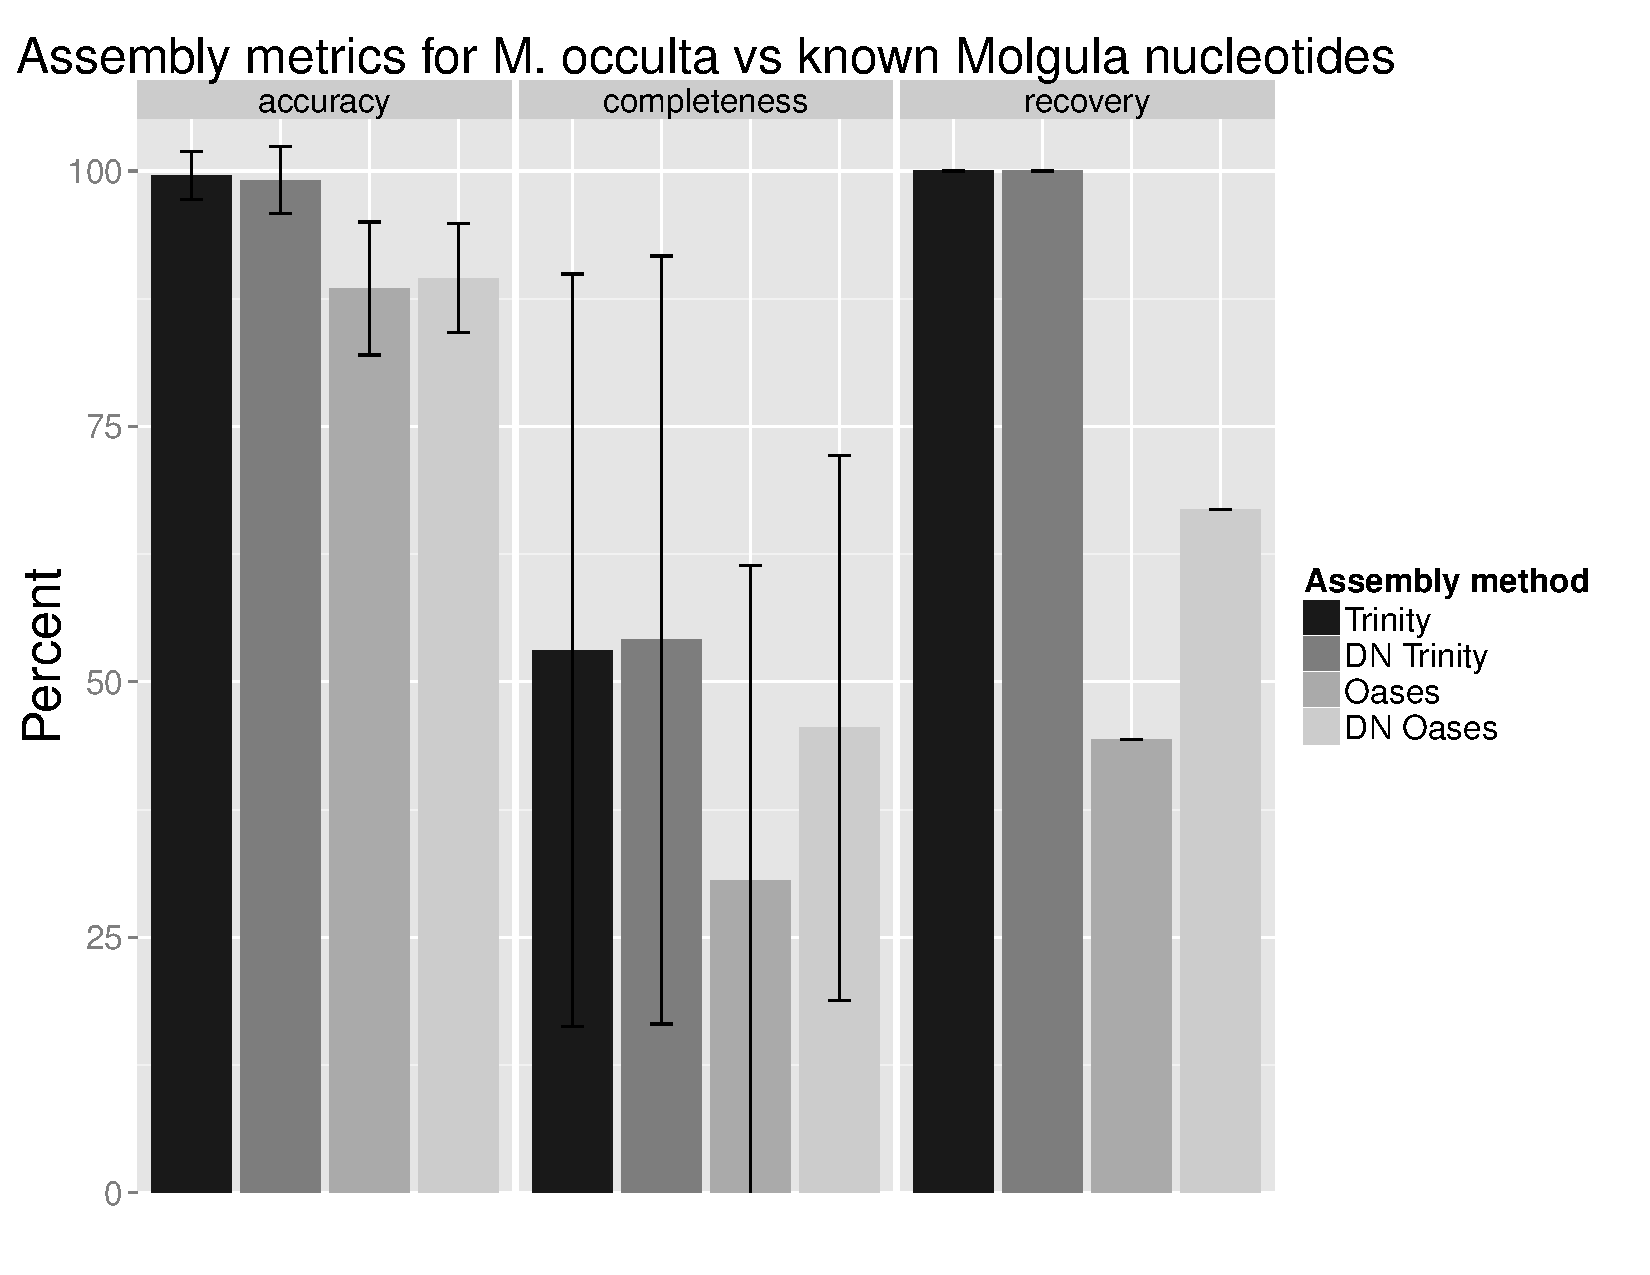
\includegraphics[width=0.4\textwidth]{manuscript/figure_4_moccVsknownmolg.pdf}
	}%
	\subfigure[]{%
                \label{fig:figure_4_mocuVsknownmolg}
                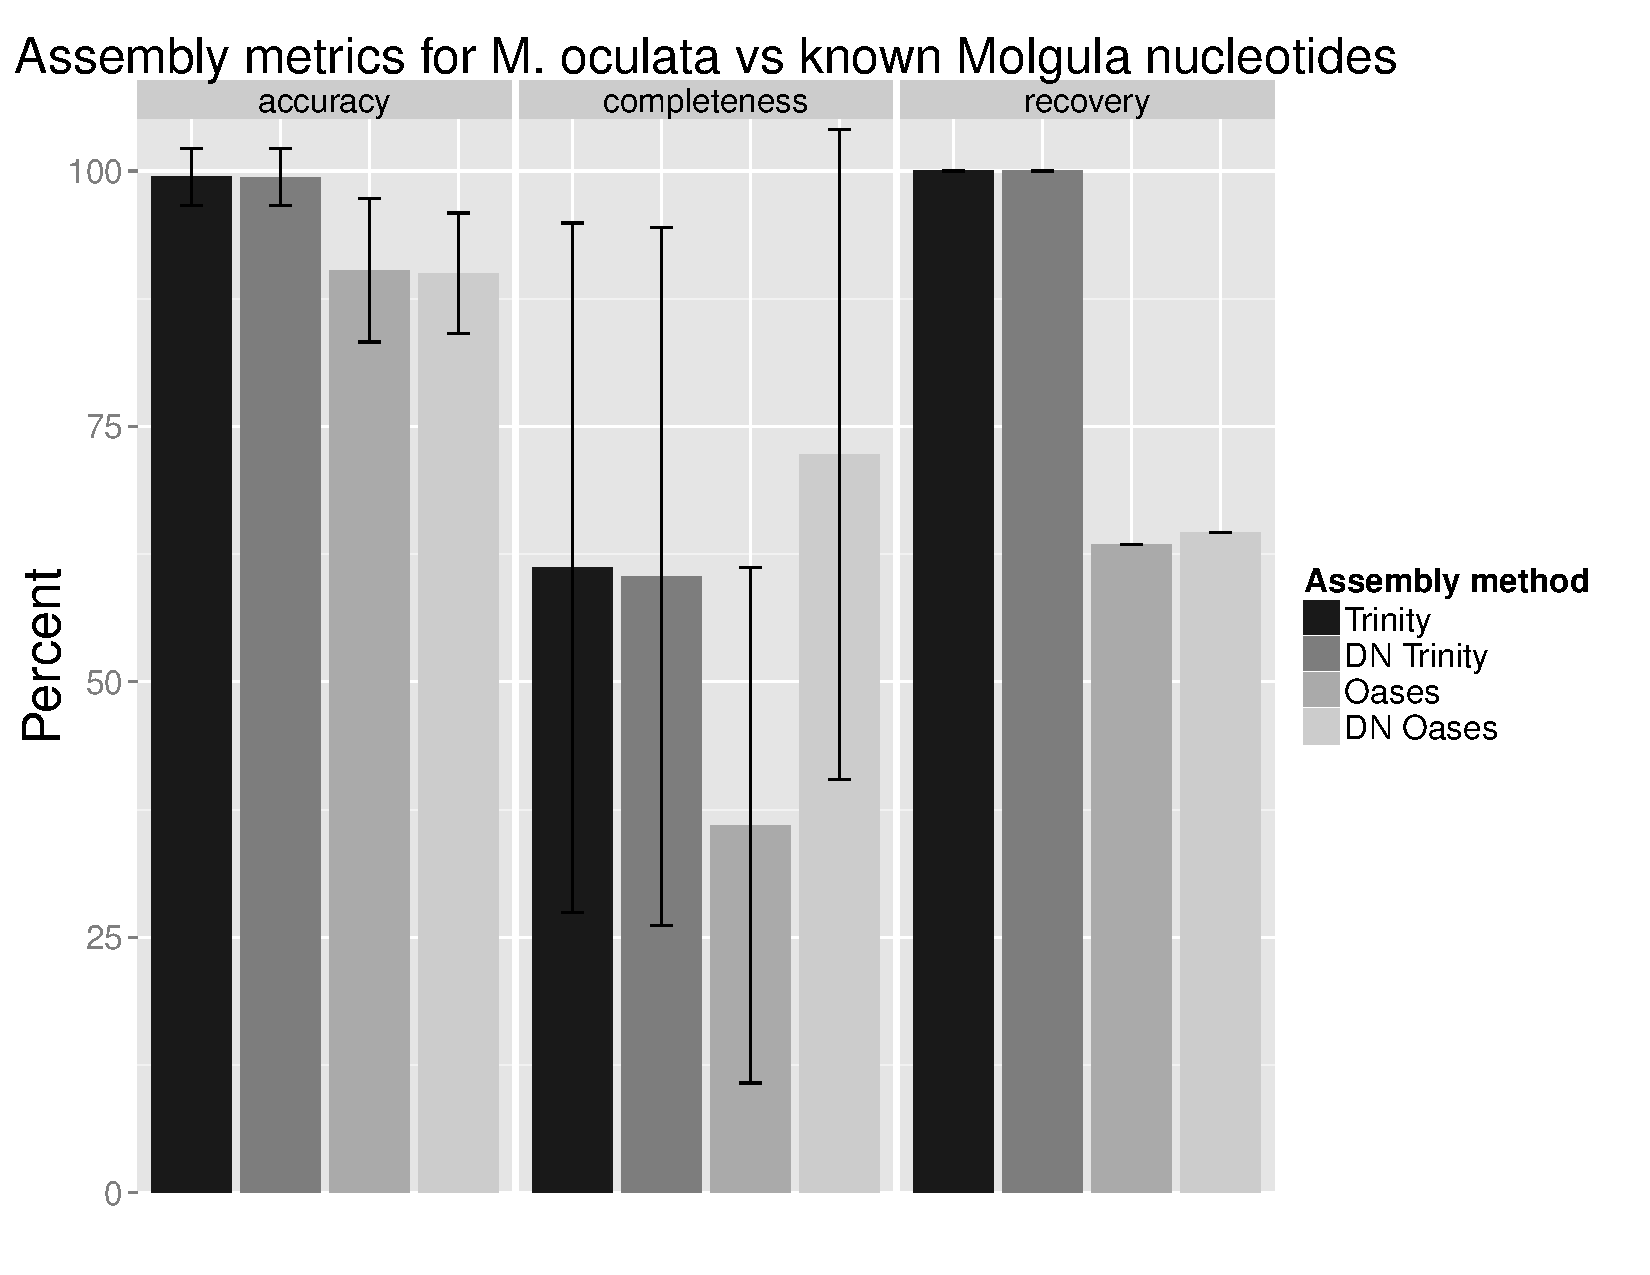
\includegraphics[width=0.4\textwidth]{manuscript/figure_4_mocuVsknownmolg.pdf}
	}%
	\end{center}
	\caption{\textbf{Accuracy, completeness and recovery rate against know Molgula sequences.} The NCBI has 178 Molgula sequence in its database. Transcripts were searched against these sequences using BLASTN with a cut-off of e-12. Trinity assemblies performed the best, recovering all known sequences. \textit{M. occulta} unnormalized assembled performed the worst, only recovering 79 (44\%) of the transcripts. \textit{M. occulta} tended to recover fewer of the known transcripts as well.}
	\label{fig:known_molg}
\end{figure}
     
Of these 178 nucleotide sequences, 8 of them are \textit{M. occulta} sequences and 15 of them are \textit{M. oculata} sequences. All \textit{M. occulta} assemblies recovered all 8 of the NCBI \textit{M. occulta} sequences with a 94\% or greater accuracy. \textit{M. oculata} assemblies recovered \textit{M. oculata} transcripts at a 93\% accuracy as well. \textit{M. occulta} assemblies produced the lowest completeness of the two species, 41\% and 43\% for unnormalized Oases and diginorm Oases respectively, and 75\% for both Trinity assemblies. \textit{M. oculata} assemblies produced more complete transcripts 66, 75, 86, and 83 percent for unnormalized Oases, Diginorm Oases, unnormalized Trinity and Diginorm Trinity respectively.


\subsection{Both unnormalized and normalized assemblies recovered many of the same transcripts}
We evaluated the two diginorm and unnormalized assemblies against one another to test whether either method missed significant portions of the transcriptome assembled by the other. We used BLAT to compare unnormalized and diginorm assemblies in both directions. In \textit{M. occulta}, both methods recovered at least 93\% of the transcripts, with Trinity diginorm recovering \mytilde99\% of Trinity's unnormalized assembly. \textit{M. oculata} assemblies showed high overlap as well, all recovering greater than 98\% of each other with the exception of diginorm Oases recovering 94\% of unnormalized Oases assembly.

\subsection{Homology search against the \textit{Ciona} proteome shows similar recovery of ascidian genes across assemblies}
We used \textit{Ciona intestinalis} to evaluate the completeness of our transcriptomes. \textit{C. intestinalis} has an assembled genome that is well annotated and is the closest available genome to the Molgulids. \textit{C. intestinalis} has a genome of ~160 Mb and contains \mytilde16,000 genes \citep{satoh_surfing_2005}. A total of 13, 835 (86\%) of the \textit{C. intestinalis} proteins found in NCBI had hits in the \textit{M. occulta} transcriptomes (Figure 5), with 2,288 genes (14\%) having no hits due presumably to either lack of expression, high divergence, or loss \textit{M. occulta}. When comparing transcripts excluded by either diginorm or unnormalized reads for all assemblies, the unnormalized read assemblies produced an additional 0.04\% hits to \textit{C. intestinalis} and there was additional 0.03\% for the diginorm assemblies. There was little difference between the assemblies when compared to \textit{C. intestinalis}, with 99\% of the \textit{C. intestinalis} genes being found in all \textit{M. occulta} assemblies (Figure 4a). Eighty-six percent of the \textit{C. intestinalis} proteins had matches in the \textit{M. occulta} and \textit{M. oculata} assemblies with less than 1\% difference in presence between the several assemblies (Figure 4b).
     
 \setcounter{subfigure}{0}
\begin{figure}[tbp]
	\begin{center}
	\subfigure[\textit{ M. occulta}]{%
                \label{fig:figure_5_mocc_blast_overlap}
                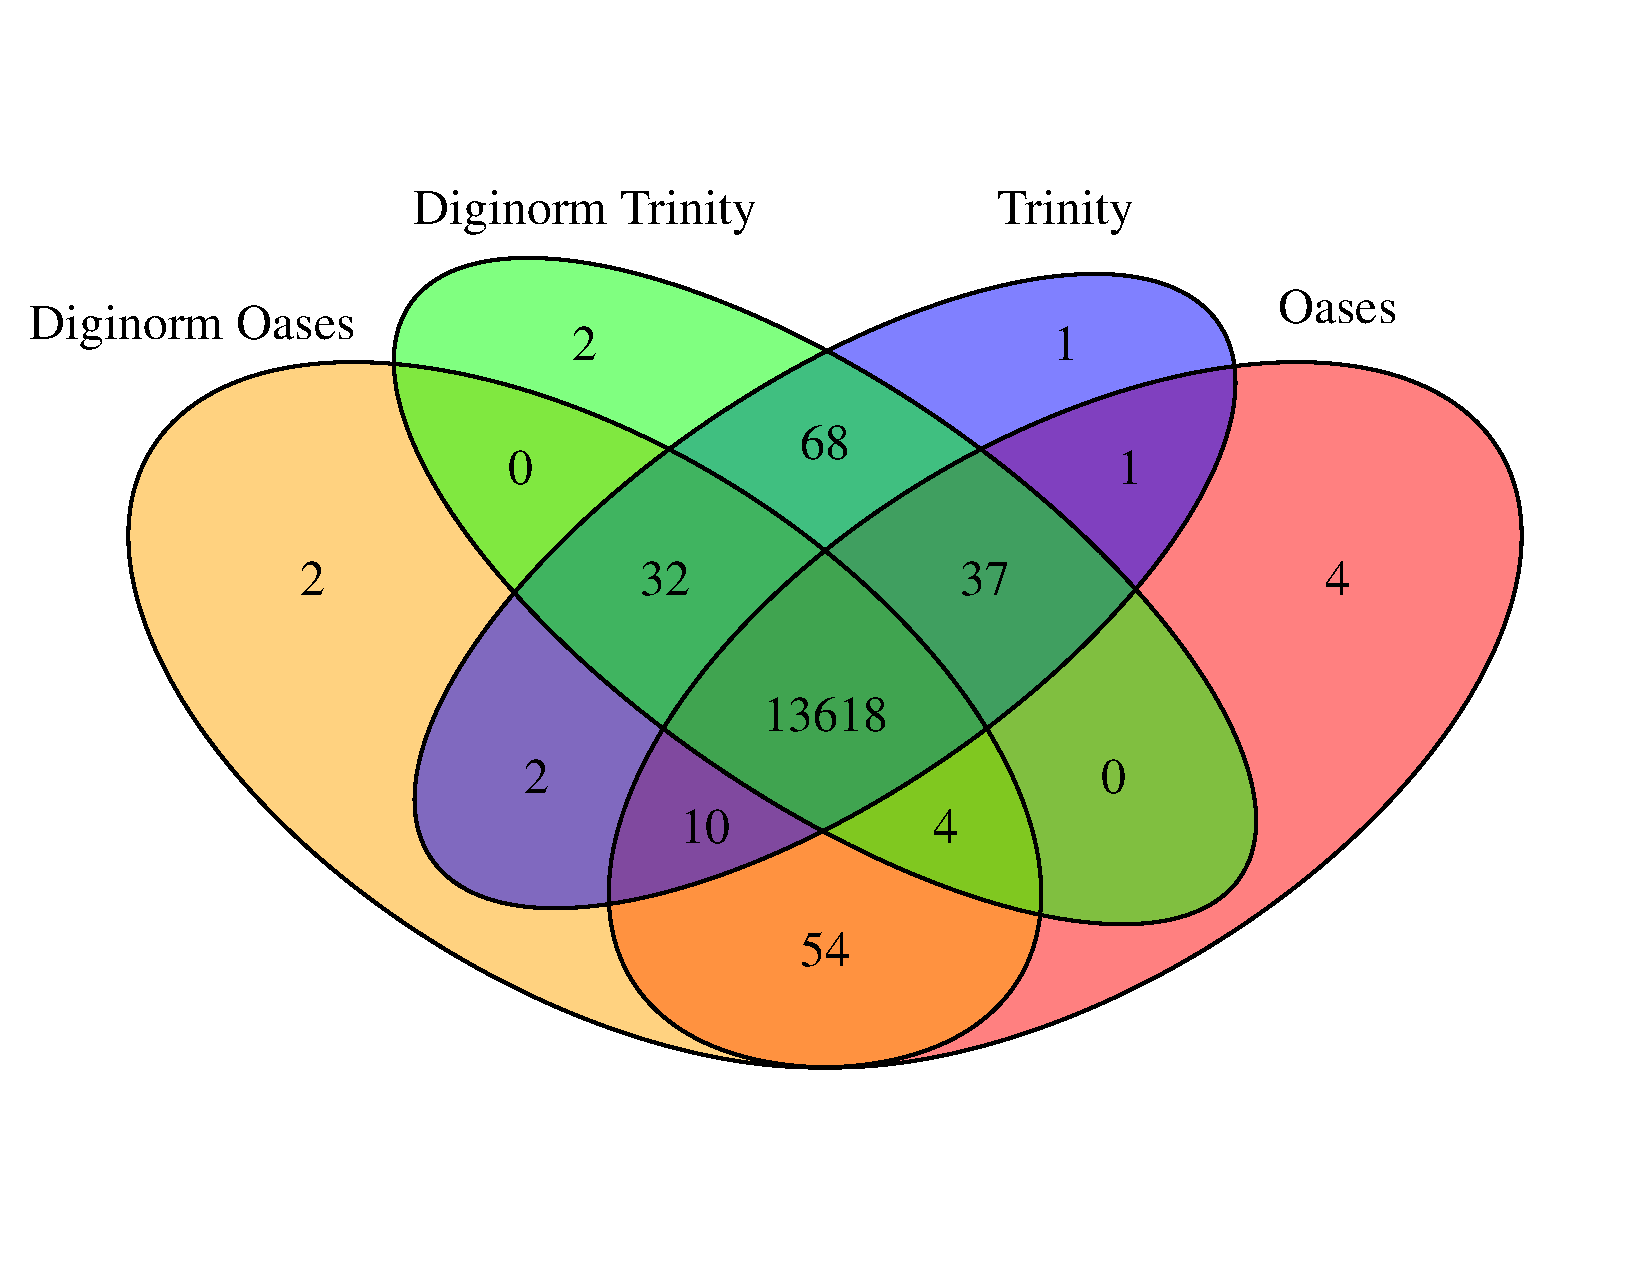
\includegraphics[width=0.4\textwidth]{manuscript/figure_5_mocc_blast_overlap.pdf}
	}%
	\subfigure[\textit{ M. oculata}]{%
                \label{fig:figure_5_mocu_blast_overlap}
                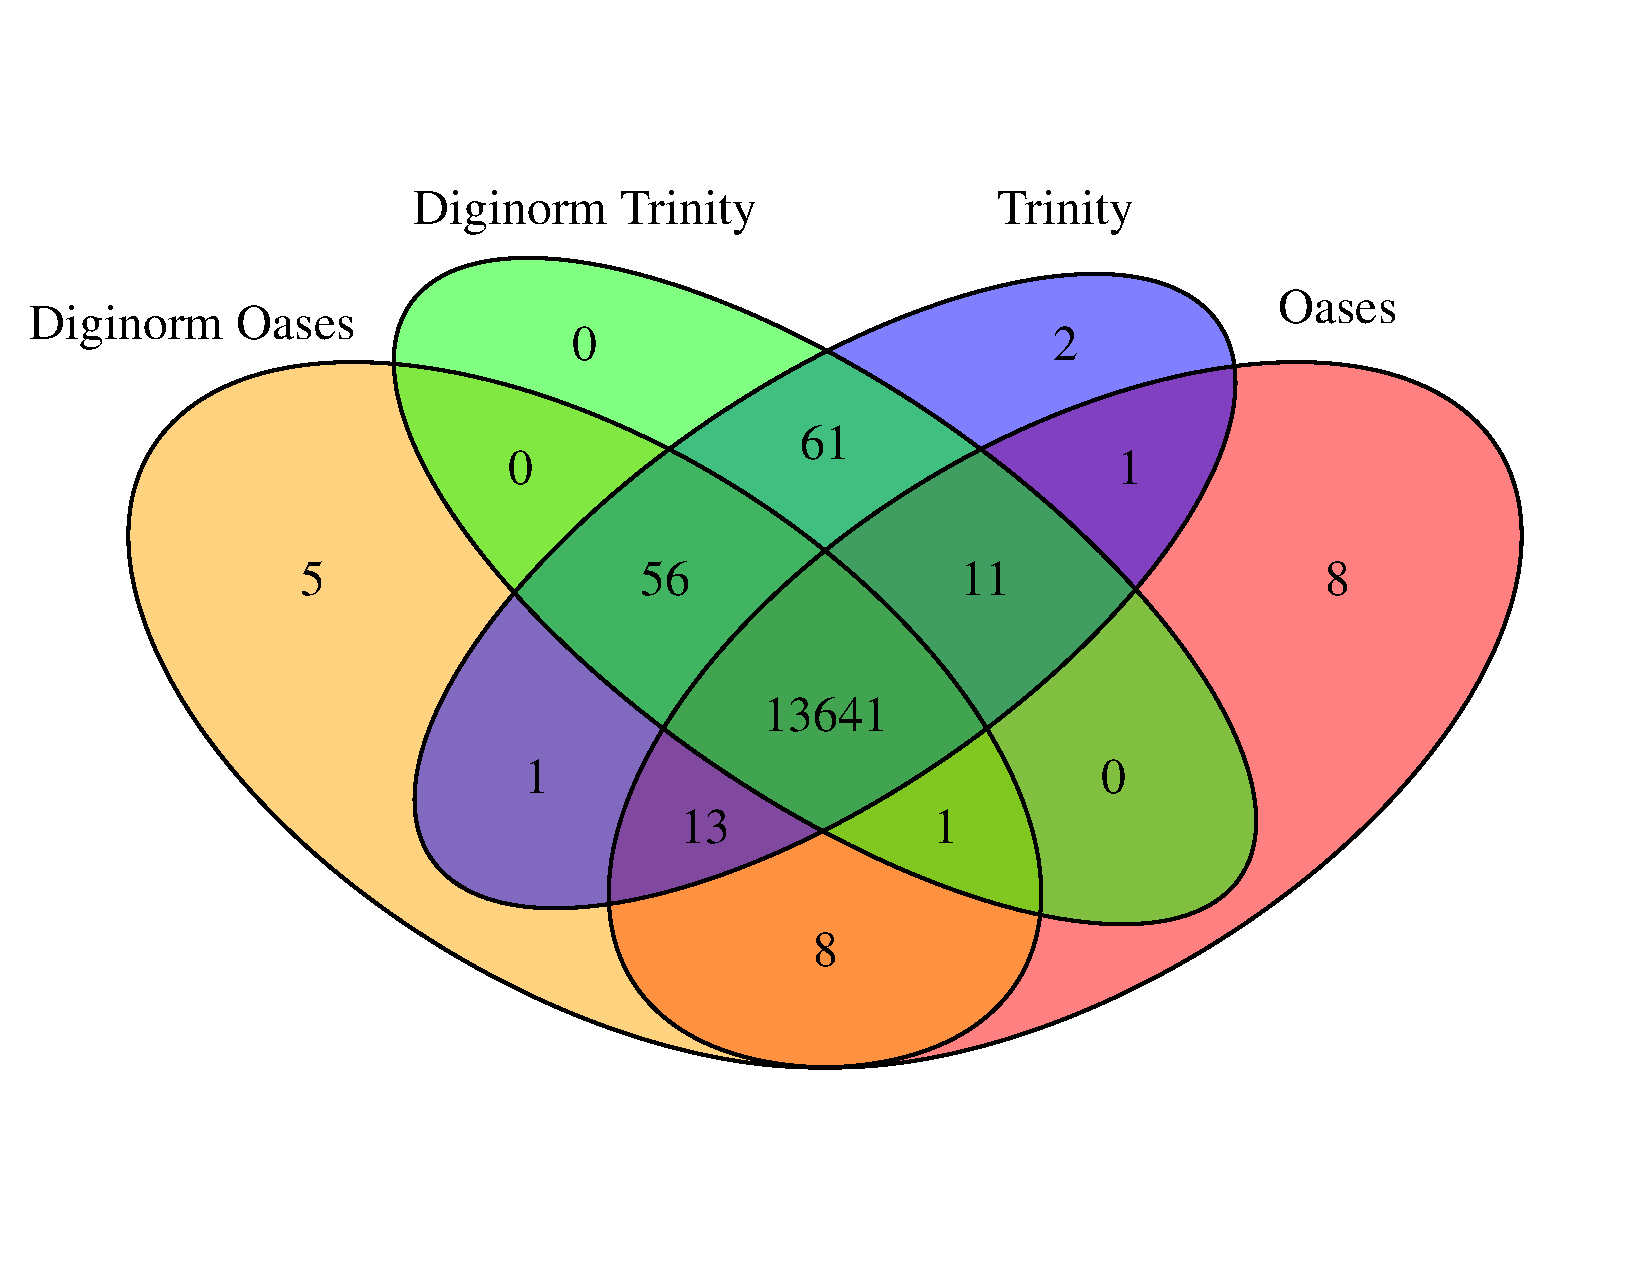
\includegraphics[width=0.4\textwidth]{manuscript/figure_5_mocu_blast_overlap.pdf}
	}%
	\end{center}
	\caption{\textbf{Gene recovery, raw reads versus normalized.} Gene homologue with \textit{C. intestinalis} via BLAST for \textit{M. occulta} (left) and \textit{M. oculata} (right). Each oval represent the total number of homologs sequences recovered. In both species the Trinity assembler assembled more homologous sequences. There was almost complete overlap in homology for both assemblers and both assembly conditions.}
	\label{fig:overlap}
\end{figure}
     
We next examined the difference between the unnormalized and digitally normalized assemblies. Transcripts in the unnormalized assembly with BLAST hits to \textit{C. intestinalis} but without hits in diginorm assemblies were extracted, and searched using BLASTN against the diginorm assemblies; we found fragmented versions of these transcripts, suggesting that they were partially assembled.  We then mapped the diginorm reads to the extracted unnormalized transcripts and found that some portions of the transcripts were not covered by the normalized reads. This demonstrates that these transcripts were lost due to a loss of information from the diginorm process.  However, the overall loss was minimal and complemented by an increase in the recovery of other conserved transcripts; this is clearly a direction for further study.
\subsection{CEGMA analysis shows high recovery of genes}
CEGMA uses a list of highly conserved eukaryotic proteins to evaluate genome and transcriptome completeness \citep{parra_cegma:_2007}. We used CEGMA to analyze the number of protein families that are present in each assembly. The default CEGMA parameters were used for analysis. CEGMA reports recovery as ``complete'' or ``partial'', where a match is marked as ``complete'' if 70\% or more of the amino acid sequence is recovered. More than 90\% of the CEGMA genes were recovered completely in each of the transcriptome assemblies, while greater than 98\% of the CEGMA genes were recovered at least partially. 

\section{Discussion}

\subsection{Transcriptome assembly accurately recovers known transcripts and many genes}

% @CTB - removed. Diginorm increased the recovery rate for the known Molgula nucleotides for the Oases assemblies. Diginorm did not have much of an effect on \textit{M. oculata}, however, \textit{M. occulta} which has 10s of millions more reads, had a much more noticeable effect, with a 51\% increase in recovered sequences. Diginorm also had a positive effect on the completeness of transcripts when assembling with Oases. Trinity performed better than Oases whether the reads are digitally normalized or unnormalized. Completeness was not over 60\% for any of the assemblies, but this is explained by the fact that most of the nucleotide sequences were not mRNA so our transcripts would not align to the intronic regions. This confirms that all assembly techniques yielded good transcriptomes when applied to both data sets.

All of the transcriptome assemblies yielded homologs for an almost identical subset of the \textit{Ciona intestinalis} proteome.  While the evolutionary distance between the Molgulids and \textit{C. intestinalis} may be large -- the Molgulids are stolidobranch ascidians and are believed to be very divergent from \textit{C. intestinalis}, which is a phlebobranch ascidian \citep{huber_evolution_2000, stach_phylogeny_2002}\textemdash approximately 84\% of \textit{Ciona} proteins were found in all assemblies via BLAST, and more than 44\% of \textit{Ciona} proteins had putative orthologs in each of our assemblies via reciprocal best hit.  Since both transcriptomes are from a limited set of embryonic tissues that do not express all genes, these are surprisingly high numbers!  We infer that we have recovered almost all embryonic genes and the majority of genes present in the Molgula genomes.

Read mapping and CEGMA analyses further confirm that the transcriptome assemblies are of high quality and inclusiveness.  The assemblies represent 75\% or more of the reads from all but one time point, contain complete matches to 90\% or more of the conserved eukaryotic gene families in CEGMA, and contain partial matches to 98\% or more of the CEGMA families.   It is important to note that the CEGMA results are almost certainly biased upwards by the nature of the CEGMA families, which represent many more metabolic and cellular function genes than e.g. animal-specific transcription factors; thus the CEGMA numbers do not directly demonstrate the inclusiveness of the transcriptome families, as they would for a genome assembly \citep{parra_cegma:_2007}.

\subsection{Digital normalization eases assembly without strongly affecting assembly content}

One of our goals in this study was explore the impact of digital normalization on the biological interpretation of transcriptome assemblies; while previous studies have shown that digital normalization can make assembly faster and less memory intensive, gene recovery has been less well studied \citep{haas_novo_2013, brown_reference-free_2012}.  Here we confirm the computational results: diginorm dramatically reduces the computational cost of Oases assemblies, and also decreases the time and memory requirements for Trinity assemblies.

While digital normalization does alter the number of transcripts significantly, it does not strongly affect either read inclusion or the conserved gene content of the assemblies. Read inclusion by mapping never decreased more than 3\% after digital normalization, and in many cases increased. The conserved gene content, measured by a proteome comparison, showed that we recover essentially the same set of proteins with all four treatments on both transcriptomes.  

Combined, these results suggest that the varying number of transcripts largely reflect differences in the splice variants reported by different assemblers under different conditions. These results also strongly support the idea that preprocessing with digital normalization does not strongly affect assembly content.  We note, however, that the few transcripts not recovered in assemblies of the digitally normalized reads were probably not recovered because the underlying reads were eliminated during digital normalization.  This is an area where digital normalization can be improved.

Only a small number (well below 1\%) of different homology matches were reported between the various assemblies.  Because of this we decided not to merge or otherwise combine the different assemblies: the likely benefits were outweighed by the risk of introducing chimeric transcripts or combining isoforms.

We also note that the variation in number of assembled transcripts due to read preprocessing and choice of assembler despite the similar gene content suggests that traditional genome assembly metrics such as number of transcripts, total bp assembled, and N50 are not useful for transcriptome evaluation as previously suggested \citep{oneil_assessing_2013}.  For example, the same exon may be included in multiple splice variants, inflating the total bp assembled; some assemblers may choose to report more isoforms than others even with the same read support; and N50 makes little sense for transcriptomes.
 
\subsection{Trinity assemblies are more sensitive to low-abundance k-mers but contain no new conserved genes}
The difference in transcript numbers between Trinity and Oases assemblies is stark: for the same data set, with the same treatment, Trinity always produces thousands more transcripts than Oases.  Moreover, many more reads can be mapped to the Trinity assemblies \textemdash an additional 10\% or more, for every stage.  Despite this greater inclusion of reads, we see no substantial gain in either CEGMA matches or \textit{Ciona} proteome matches for the Trinity assemblies.

This conundrum can be resolved by examining the k-mer spectra, which show that the Trinity assemblies include many more low-abundance k-mers from the read data set.  This demonstrates that Trinity is more sensitive to low-abundance sequences, and may include more isoforms in its assemblies\textemdash by design, Trinity attempts to be more sensitive to isoforms than Oases, and focuses particularly on low-coverage isoforms \citep{vijay_challenges_2012, grabherr_full-length_2011, van_belleghem_novo_2012}. Those transcripts were indeed the results of Trinity assembling low coverage reads, having an average coverage of 5x compared to 75x.
 
\section{Conclusions}
We show that transcriptome assembly on two closely related species of Molgulid ascidians produced accurate and high-quality transcriptomes, as determined by several different metrics.  Importantly, four different assembly protocols produced transcriptomes that contained nearly identical complements of homologs to the nearest model organism, \textit{Ciona intestinalis}.  While variations in isoform content were observed, these variations had little apparent impact on sensitivity of homologous gene recovery. We provide detailed assembly protocols that should enable others to easily achieve \textit{de novo} transcriptome assemblies.

\section*{Acknowledgments}

EKL and this research were supported by the National Science
Foundation under Cooperative Agreement No. DBI-0939454 (BEACON). Any
opinions, findings, and conclusions or recommendations expressed in
this material are those of the authors and do not necessarily reflect
the views of the National Science Foundation.  CTB was supported in
part by Agriculture and Food Research Initiative Competitive Grant
no. 2010-65205-20361 from the United States Department of Agriculture,
National Institute of Food and Agriculture.


\chapter{Genome assembly and characterization}
\section{Introduction}
Ascidians are marine invertebrates that spend their adult life filter feeding through an incurrent siphon and an outcurrent siphon. Ascidians are evolutionarily interesting because of the phylogentic position\textemdash urochordates\textemdash the sister group to vertebrates and cephalochordates, together they form the chordate phylum. Although ascidans share no resemblance to vertebrates in their adult stage, they share several features, a notochord, dorsal hollow neural tube, and gill slits during development in addition to 18S placement \cite{wada_details_1994, Cameron et al 2000}. The development of ascidians are well documented, the cell lineage from fertilization to gastrulation has be followed in \textit{Ciona intestinalis} \cite{nishida_cell_1983,nishida_cell_1985,nishida_cell_1987}. Studies of other ascidians species have shown that the majority of phyla has an invariant cell lineage and typical development \cite{berrill_studies_1931}. Only very few solitary ascidians have deviated and undergone tail-loss \cite{swalla_interspecific_1990, tsagkogeorga_updated_2009}. \textit{M. occulta} and \textit{M. oculata} are two species that are found in the shallow waters for Roscoff, France that closely resemble each other in their adult stage, they differ only by a white pigment spot found between the siphons of \textit{M. oculata} Figure~\ref{fig:adults}. These two text it{Molgula} species, however, have different methods of development\textemdash \textit{M. oculata} developing a typical tadpole larvae and \textit{M. occulta} developing without a tail. Many of the genes have been studied across a number of ascidian, showing that gene function tends to be orthologous within the phyla \cite{satoh_ascidian_2003}. 

although genes tend to be expressed in homolguous patterns and tissues, the presence of gens are not the same across species . there has also been cases where genes that have been shown to be important for important biological process are absence in spies why the affected phonotype. it has also been shown that in ascidians with the same phenotype and gene expression, regulatory modules are not necessarily the same. Ascidian speices are far more divergent than the appear phenotypicaly. Genomics has shed some light on the area. because ascidians are board cast spawners they are highly polymorhpic and has rapid rates of evolution. this has cause fairly divergence genomes outside of coding regions. we will demonstrate this using closely related speices and more divergent \textit{M. occidentalis}. Whole genome sequencing and assembly has given us a better picture of what is going on evolutionary for close and divergent species. we are about to charaterize gene networks, identify regulatory elements and get a better understanding of something that sounds really important. here we use next-generation sequencing to compare the genomes of three molgula spp and to charaterize the hox clusters of those spp.

However, as with most biological processes there is  there are cases where gene expression differences led to variation, in addition to genes with important functions . Genomics allows us to identify elements involved in the 
regulation of genes. To identify elements of such, information for a number of species 

Ciona intestinalis was the first ascidian species to be sequenced

\begin{figure}[tbp]
\centering
\includegraphics[scale=0.5]{figures/adults.pdf}
\caption{\textbf{Adult ascidians.} \textit{M. occulta} (A) and \textit{M. oculata} (B) are nearly identical in their adult stage with the white pigment spot (red arrow). Their tunic is covered in sand, seeing that they are found on the sandy sea bottoms. Under there sand covered tunic, the two species differ by the color of their eggs\textemdash purple in \textit{M. oculata}, pictured and an orange-yellowish color in \textit{M. occulta}\textemdash found just above the kidney complex (C). \textit{C. intestinalis} (D) is one of the more studies ascidians and has a assembled genome.}
\label{fig:adults}
\end{figure}

\section{Materials and methods}

\subsection{Genomic DNA library preparation and sequencing}
Genomic DNA was phenol/chloroform extracted from dissected gonads of \textit{Molgula occulta} (Kupffer) and \textit{Molgula oculata} (Forbes) adults from Roscoff, France, and a \textit{Molgula occidentalis} (Traustedt) adult from Panacea, Florida, USA (Gulf Specimen Marine Lab). Genomic DNA was sheared using an M220 Focused-ultrasonicator (Covaris, Woburn, MA). Sequencing libraries were prepared using KAPA HiFi Library Preparation Kit (KAPA Biosystems, Wilmington, MA) indexed with DNA barcoded adapters (BioO, Austin, TX). Size selection was performed using Agencourt (Beckman-Coulter, Brea, CA) AMPure XP purification beads (300-400 bp fragments), or Sage Science (Beverly, MA) Pippin Prep (650-750 bp and 875-975 bp fragments). For \textit{M. occulta} and \textit{M. occidentalis} libraries, 6 PCR cycles were used. For \textit{M. oculata} libraries, 8 cycles were used for the 300-400 bp library, and 10 cycles were used for the 650-750 and 875-975 bp libraries. Libraries of different species but same insert size ranges were multiplexed for sequencing in three 100 � 100 PE lanes on a HiSeq 2000 sequencing system (Illumina, San Diego, CA) at the Genomics Sequencing Core Facility, Center for Genomics and Systems Biology at New York University (New York, NY). Thus, each lane was dedicated to a mix of species, specifically barcoded libraries of a given insert size range. Raw sequencing reads were deposited as a BioProject at NCBI under the ID\# PRJNA253689.
\subsection{Genome sequence assembly}
All genomes were assembled on Michigan State University High Performance Computing Cluster (http://contact.icer.msu.edu). Prior to assembly, read quality was examined using FastQC v0.10.1. Reads were then quality trimmed on both the 5' and 3' end using seqtk trimfq (https://github.com/lh3/seqtk) which uses Phred algorithm to determine the quality of a given base pair. Seqtk trimfq only trims bases, so no reads were discarded. Each library per species was then abundance filtered using 3-pass digital normalization to remove repetitive and erroneous reads \cite{brown_reference-free_2012,schwarz_genome_2013}, Howe et al., 2014). Genome assembly was done using velvet v1.2.08 \cite{zerbino_velvet:_2008} with k-mer overlap length (`k') ranging from 19 to 69 and scaffolding was done by Velvet, by default. Velvet does not produce separate files for contigs and scaffolds; because Velvet scaffolded conservatively, contigs dominated the assemblies so we refer to both contigs and scaffolds as contigs. CEGMA scores were then computed to evaluate genome completeness \cite{parra_cegma:_2007}. The latest versions of three species' genome assemblies have been deposited on the ANISEED (Ascidian Network for In Situ Expression and Embryological Data) database for browsing and BLAST searching at http://www.aniseed.cnrs.fr/ \cite{tassy_aniseed_2010}. Scripts for genome assembly and CEGMA analysis can be found in the following github repository: https://github.com/elijahlowe/molgula\textunderscore genome\textunderscore assemblies.git
\subsection{Gene identification and alignments}
Thirty-nine hox genes were identified in hunman and downloaded from the NCBI database. These sequences were then BLAST against each of the three assembled \textit{Molgula} genomes. The alignments were then extracted BLAST against the NCBI non-redundant database. \textit{Molgula} alignments sequences were extracted, annotated and placed in the following files, mocc\_hox\_aa.fa, mocu\_hox\_aa.fa, and moxi\_hox\_aa.fa, which are located ???. Hox1-13 sequences for human, fruit fly, and Amphioxus were download from `Homeobox Database' (http://homeodb.zoo.ox.ac.uk/). These sequences were then joined with the identified Molgula \textit{hox} genes and used to produce a phylogenetic trees using MAFFT version 7 online rough tree program at http://mafft.cbrc.jp/alignment/server/clustering.html \cite{katoh_parttree:_2007,katoh_mafft_2013}.  Additional alignments between the three species were conducted using mVista \cite {mayor_vista_2000,frazer_vista:_2004,visel_vista_2007} with \textit{M. oculata} as the anchoring sequence because it shows the most similarity between the three \textit{Molgula} species. The LAGAN alignment algorithm was used with translated anchoring to improve alignment because of evolutionary distances\cite{brudno_lagan_2003}.    

\section{Results}
\subsection{Genome assemblies assessment}
Genomes of three Molgula species (\textit{M. occidentalis}, \textit{M. oculata}, and \textit{M. occulta}) were sequenced using next-generation sequencing technology and assembled. A common metric for judging the quality of a genome assembly is the contig N50 length, which is determined such that 50\% of the assembly is contained in contigs of this length or greater. We used the contig N50 length to select the best assembly for each species given the varying `k' parameter (length of k-mer overlap). A `k' of 39 yields the best assembly for both \textit{M. occidentalis} and \textit{M. occulta}. The best `k' for \textit{M. oculata} was 61. \textit{M. occidentalis}, \textit{M. occulta}, and \textit{M. oculata} N50 lengths were approximately 26.3 kb, 13 kb, and 34 kb, respectively (Table 1).
\begin{table}[tbp]
\centering
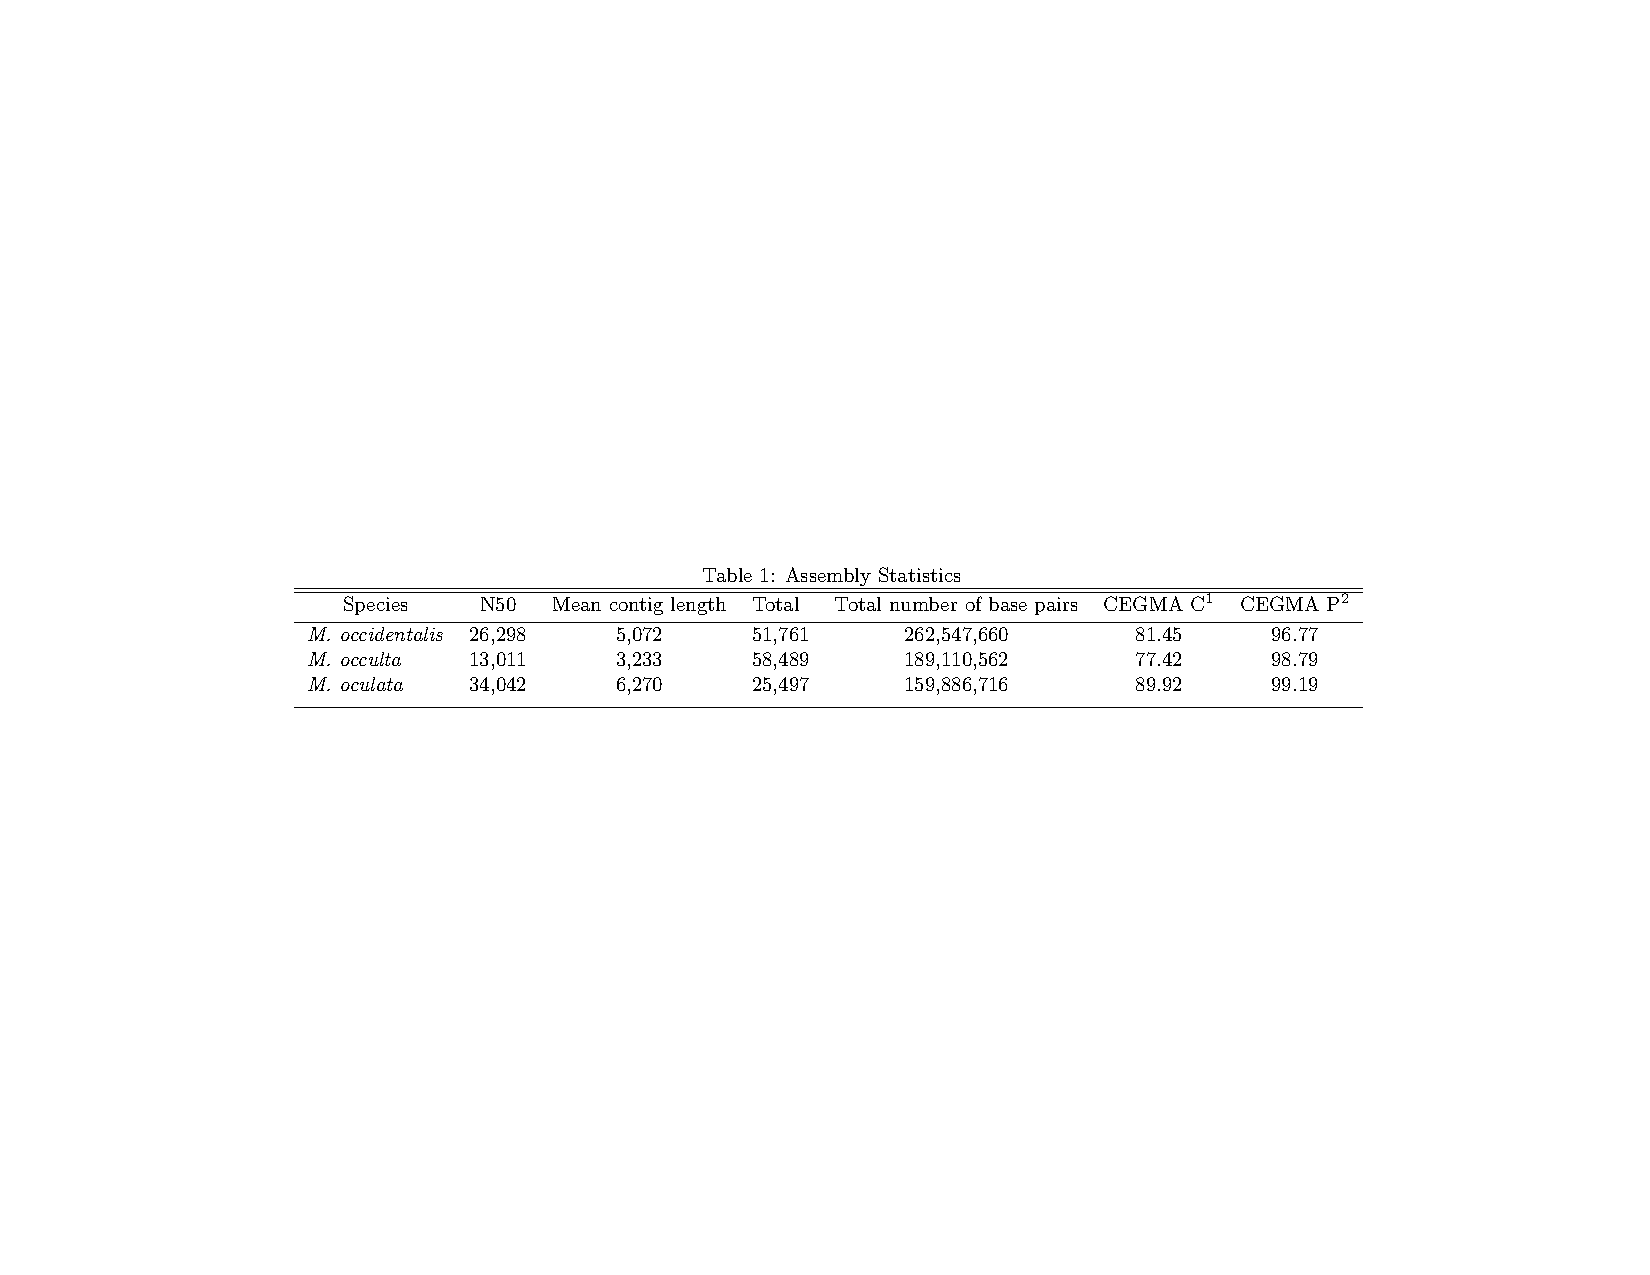
\includegraphics[width=\linewidth]{figures/genome_table_1}
\caption{\textbf{Digitally normalized reads.} The number of reads sequenced before and after digital normalization are shown for each lane of sequencing. The percentage of total reads kept after digital normalization is shown in bold. \textit{M. occulta} had approximately \mytilde237 million reads and was reduced to 91 million reads, a 60\% reduction. \textit{M. oculata} had 150 million reads and reduced by 77\% to \mytilde50 million reads. }
\label{table:genome_table}
\end{table}
In addition to N50 lengths, we also used CEGMA (Core Eukaryotic Genes Mapping Approach) scores, in order to evaluate the assemblies' representative completeness (Parra et al., 2007). CEMGA reports scores for complete and partial alignments to a subset of core eukaryotic genes. An alignment is considered ``complete'' if at least 70\% of a given protein model aligns to a contig in the assembly, while a partial alignment indicates that a statistically significant portion of the protein model aligns. The partial alignment scores are \mytilde97\% or higher for all assemblies. \textit{M. oculata} has the best complete alignment score at \mytilde90\%. \textit{M. occidentalis} and \textit{M. occulta} have complete alignment scores of 81\% and 77\% respectively (Table 1). These scores indicate that our assemblies contain at least partial sequences for the vast majority of protein-coding genes in the genomes of these species.
Various factors make it unreliable to predict genome size and gene density based on assembly metrics alone (Bradnam et al., 2013). Of the handful of sequences we isolated and analyzed, we found that the sizes of introns and upstream regulatory regions were roughly comparable to those from their \textit{Ciona} orthologs. This suggests that the \textit{Molgula} genomes may be as compact as the \textit{C. intestinalis} genome (i.e., \mytilde150-170 Mb, \mytilde16,000 genes, Laird, 1971; Simmen et al., 1998; Satou et al., 2008).
\subsection{Divergence of GRN}
Our sequencing efforts revealed extreme genetic divergence not only between \textit{Ciona} and \textit{Molgula}, as expected, but even within the Molgulids. For example, we used BLAST to identify the \textit{Molgula} orthologs of \textit{C. intestinalis Mesp} (\textit{Ciinte.Mesp}, as per the proposed tunicate gene nomenclature rules, see Stolfi et al., 2014). \textit{Ciinte.Mesp} is the sole ortholog of vertebrate genes coding for \textit{MesP} and \textit{Mesogenin bHLH} transcription factor family members (Satou et al., 2004). VISTA alignment shows high sequence similarity between sequences 5' upstream of the \textit{Mesp} genes from the closely related \textit{M. oculata} and \textit{M. occulta} (Figure 1B). However, there is no conservation of \textit{Mesp} DNA sequences, coding or non-coding, between \textit{M. oculata}/\textit{occulta} and \textit{M. occidentalis}, nor between \textit{C. intestinalis} and any of the three \textit{Molgula} species (Figure 1?figure supplement 1). In previous phylogenetic surveys, \textit{M. occidentalis} has been placed as an early-branching \textit{Molgula} species, often grouped together in a subfamily with species ascribed to the genera Eugyra and Bostrichobranchus instead (Hadfield et al., 1995; Huber et al., 2000; Tsagkogeorga et al., 2009). Our sequencing results support the view that \textit{M. occidentalis} is highly diverged from other \textit{Molgula} spp.

\begin{figure}[tbp]
\centering
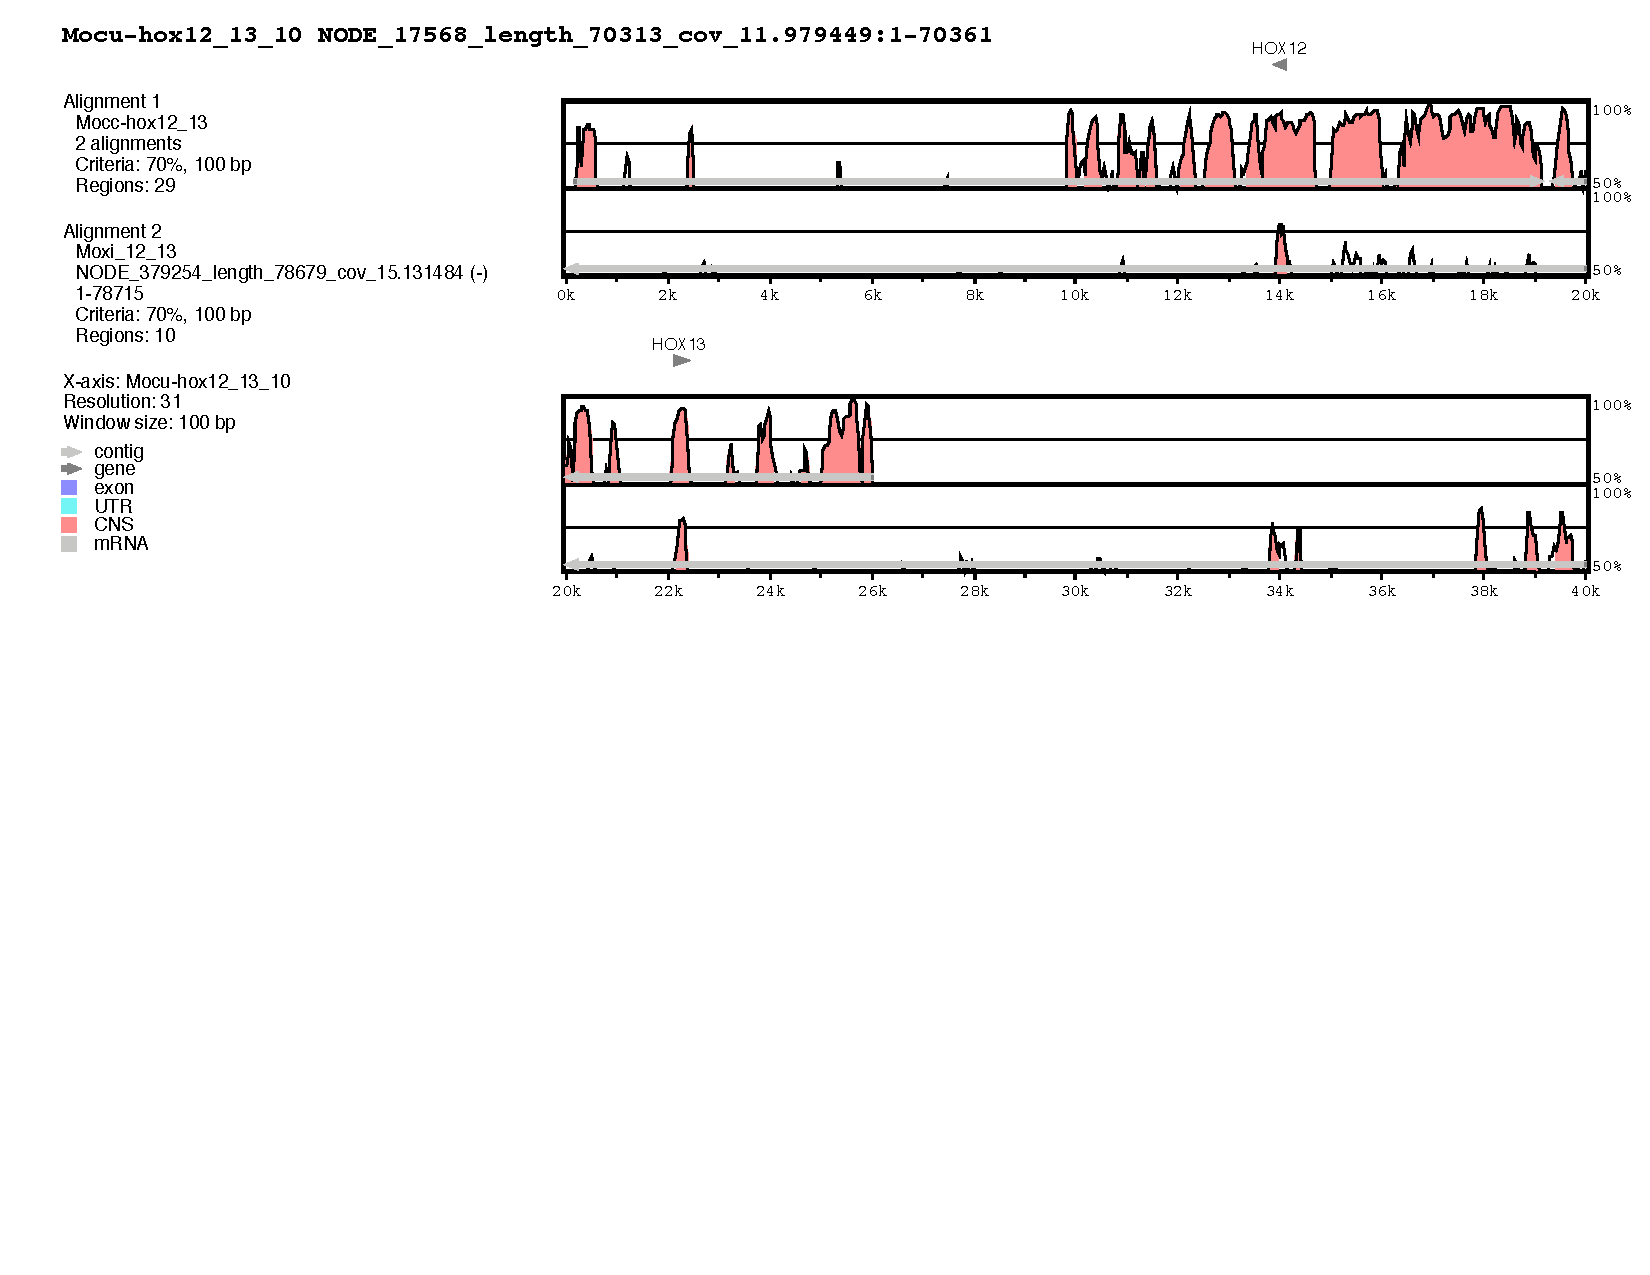
\includegraphics[scale=0.55]{figures/Hox12_13.pdf}
\caption{\textbf{Hox cluster for \textit{Hox 10, 12-13} in \textit{M. occulta}, \textit{M. oculata} and \textit{M. occidentalis}} }
\label{fig:hox12}
\end{figure}
\subsection{Gene complexes}
When studying development it is important to characterize the genome for particular gene cluster/families. There are 4 HOX clusters in humans  totaling in 39 genes. Within tunicates, \textit{C. intestinalis}, \textit{Halocythia roretzi} and text it{Oikopleura dioica} \textit{hox} genes have been characterized. \textit{C. intestinalis} has 9 hox genes, Hox1 through 6, Hox10, and Hox12-13 \cite{dehal_draft_2002}. The hox gene of \textit{C. intestinalis} where initially found on 5 scaffolds spanning \mytilde{980} kb using the draft assembly, with \textit{hox2-4}, \textit{hox5-6} and \textit{hox12-13} being found on the same scaffold.  two clusters of hox genes across two chromosomes \cite{ikuta_ciona_2004}. \textit{O. dioica} also has 9 hox genes, hox1-2, hox4, a duplicate hox9, and hox10-13, however, none of the genes have been found on the same scaffold, even using a 250 kb window \cite{siok_biological_2004}. Eight hox genes have be found in \textit{M. occulta} and \textit{M. oculata}, while nine have been found in \textit{M. occidentalis}. Hox1, hox2, hox3-4, hox5, hox10 and hox12-13, with hox3-4 being found on the same contig in all three species. Additionally hox10, and hox12-13 are found on the same contig in \textit{M. oculata} with only \textit{hox12-13} being found on the same contig in \textit{M. occidentalis}. However, it appears that the hox genes have been rearranged and hox10 is downstream of hox12-13 in \textit{M. oculata}. Hox12-13 are not found on the same contig in \textit{M. occulta}, however when aligned with mVista there appears to be a strong case for synteny (Figure~\ref{fig:hox12}). \textit{M. occidentalis} had one additional \textit{hox} gene compared to \textit{M. occulta} and \textit{M. oculata}, there appears to be a duplicate \textit{hox10} gene \mytilde12kb apart found on the same contig. M. occidentalis hox genes span across 5 contigs, hox2 has a stop codon located in the 3-4 helix. 

There is very little synteny between M. occulta, M. oculata and M. occidentalis. When looking at the hox complex for both hox3-4 and hox12-13, only in coding regions does there appear to be syntyany.  

Ciona exhibits longer and than usual introns between hox genes, averaging in the 5Mb range, when typically the hox genes have 100-120 kb separating them \cite{McGinnis 1992}
Because of the lack of homology outside of coding regions, we were able to identify distaless location downstream of hox13 in both M. occidentalis and M. oculata, this was not the case for M. occulta. 
\begin{figure}[tbp]
\centering
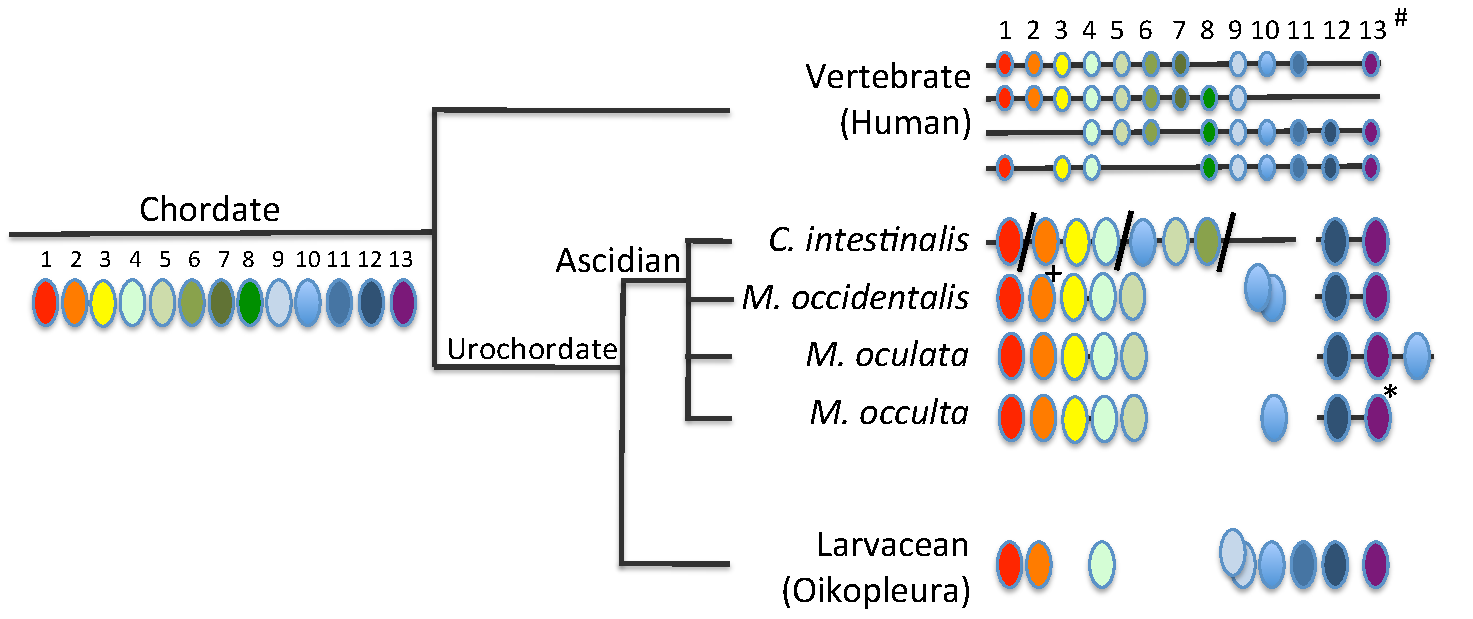
\includegraphics[scale=0.65]{figures/hox.pdf}
\caption{\textbf{Hox cluster for \textit{Hox 10, 12-13} in \textit{M. occulta}, \textit{M. oculata} and \textit{M. occidentalis}} }
\label{fig:hox12}
\end{figure}

\section{Discussion and Conculsion}
Three molgula species have been sequenced and assembled, this is the first of any molgulides to have genomes. 
\chapter{Another chapter}

\chapter{Conclusions}
The chordate body plans is fairly conserved throughout the phyla, with most developing into a tadpole larvae containing a hollow dorsal neural tube, and a postanal tail containing a notochord flanked by muscle cells. Molguilds are especially useful models because for studying the development of body plans because they have both tailed and tail-less species, two of which has the ability to produce interspecific hybrids. This allows us to examine the mechanisms of evolutionary divergent body plans at an allele-specific level. 

\section{Evaluating a lightweight transcriptome assembly pipeline on two closely related ascidian species}
Many non-model systems are now being sequenced with the drop in sequencing price. The methodology for assembly is not cut and dry, there are number step\textemdash quality trimming, filtering, choice of assembler and metrics to evaluate assembly. One of the standard is the N50, which has been designed for genomes and does not clearly translate to transcriptomes because of their fragmented nature, and the likelihood of chimeric contigs. We show that pre filtering quality trimmed assembly reads does not reduce the information content of the assembly. Many times assembly methods are chosen on the usability of software and the availability of resources. We have demonstrated that the Oases and Trinity assemblers returns similar results, suitable for downstream analysis. Our pipelines are available so we also provide methodology to be used by future researchers. 

\subsection{Contributions}
The experimental design for the RNA sequence analysis was decided by C. Titus Brown (CTB) and Billie J. Swalla (BJS). The fertilization and collection of RNA samples were done by BJS and myself. Library preparation for Illumina sequencing was done by Kanchan Pavangadkar. All downstream analysis was done by myself. The idea for evaluating de novo assembly pipeline came about through conversations with CTB, as well as methods for evaluation the transcriptome assemblies. Writing was done by me with edits from BJS and CTB.

\section{Genome assembly and characterization}
\subsection{Contributions}
The experimental design for the DNA sequencing was decided by CTB, BJS, and Lionel Christiaen (LC). Embryonic samples were collected by BJS, LC, Alberto Stolfi (AS), Claudia Racioppi (CR) and myself. Genome assembly was conducted by me. Ideas for examining divegand were developed by AS, orthologous sequences were identified through the use of RBH blast and done so by me because the sequences were not yet search about on the Aniseed database. The \textit{Hox} analysis was done by me and was conduced because of a question from David Arnosti. Writing was done by AS, myself with edits from BJS, CTB, CR, and LC.

\section{Differential expression analysis of tail loss in an invertebrate chordate}
Studying closely related organisms gives us insight into the underlying evolutionary mechanisms of divergence and underlying development. Indirect and direct developing sea urchins have been studied showing that change in axis and cell fate leads to divergent larval body plans that exhibits similar adults \cite{}. In contrast, ascidians retain their typical cell division and invariant cell fate. This is evident in both direct and indirect tail-less ascidians \cite{}. 
\subsection{Contributions}
The experimental design is the same for the "Evaluating a lightweight transcriptome assembly pipeline on two closely related ascidian species" chapter (3). Transcript models were assembled by me. Read mapping for differential expression analysis was conducted by me, and the analysis of hybrid expression counts were the idea of CTB. The differential expression analysis was conducted by me, including the idea to focus on the overlapping upregulated gene in \textit{M. oculata} and the interspecific hybrid. Annotation of the overlapping upregulated genes was done by AS, Anna Di Gregorio and myself. Writing was done by me with edits from AS, CR, and CTB.
  
Next generation sequencing is a great way to study non-model species. A broad swath of information can be gained from both RNA and DNA sequencing. This technology has allowed us to analyzed two closely related invertebrate chordates that also hybridize. This study has given us insight into the mechanisms behind tail-loss and development. Gene loss has occurred but other factors appear to be involved in tail-loss because expression from the tailed species appears to recover the loss features. 


%%%%%%%    APPENDICES    %%%%%%%%%%
%% If you wish to include one appendix, remove the "%" from the 
%% following two lines.
\renewcommand{\appname}{APPENDIX}
\appendix
ascidian
notochord
tunicate
NGS
rna-seq
de novo assembly
mapped based assembly
urdele
anural
M. occulta
M. oculata
M. occidentalis
C. intestinalis

%% To include several appendices, remove the only the "%"
%% in front of "\appendix".

%% In either cast to start your first appendix, which will be labeled
%% as Appendix A, just type \chapter{<appendix 1 name>}
%% and enter the text of the appendix as you would a chapter.

%%%%%%% A NOTE ABOUT APPENDICES %%%%%%%%%
%% Some appendices may be single spaced such as survey examples or letters.
%% Contact the Graduate School for details.
%% To single space an appendix first remove the % from 
%% the following two lines. 
% \end{doublespace}
% \chapter{<appendix  name>}
%% After entering the appendix remove the % from 
%% the following line
% \begin{doublespace}
%% Any text entered now will be double spaced.
\end{doublespace}

%%Bibliography 

%% A bibliography is required. By default it is called, "Bibliography"
%% You may use �Literature Cited�, �Works Cited� or �References� 
%% instead of �Bibliography� if that is the convention in your discipline. 
%% To do so, place your choice in the  empty argument 
%% of the following command and remove the "%".
\renewcommand{\bibname}{BIBLIOGRAPHY}
%% The bibliography may be made using BibTeX.
%% If it's made from scratch,
%% remove the "%" in front of "\begin{thebibliography}{???}"
%% replacing the ??? with the appropriate entry and 
%% remove the "%" in front of "\end{thebibliography}"
% \begin{thebibliography}{???}
%%  Enter the bibliography here.
% \end{thebibliography}

\bibliographystyle{abbrv}
\bibliography{MyLibrary}

\end{document}
